\documentclass[english]{abarbeit}
% If you write in English, set the option "english" instead of "german".
%%%%%%%%%%%%%%%%%%%%%%%%%%%% Zusätzliche Pakete
% Notizen, mit "disable" ausblendbar
\usepackage[textsize=scriptsize]{todonotes}
% Für Grafiken per latex-code bspw. TikZ und pgfplots:
\usepackage{tikz}
\usepackage{pgfplots}
\usepackage{float}
\usepackage{graphicx}
\usepackage{amssymb}
\usepackage{acro}
\usepackage{multirow}
\usepackage{subcaption}
\usepackage{adjustbox}
\usepackage{pdflscape} % falls querformat
\usepackage{pdfpages}
\usepackage[table]{xcolor}
\def\checkmark{\tikz\fill[scale=0.4](0,.35) -- (.25,0) -- (1,.7) -- (.25,.15) -- cycle;}
% Pseudocode bspw. eines der folgenden Pakete, nach Wahl
%\usepackage[plain,chapter]{algorithm}
%\usepackage{algorithmic}
%\usepackage{algorithm2e}
% minted: Syntaxhighlighting, benötigt aber pygmentize
%\usepackage{minted}
\usepackage{fancyvrb} % für pygment-Beispiele
\fvset{listparameters=\setlength{\topsep}{0pt}\setlength{\partopsep}{0pt}} % Abstände bei Verbatim vermeiden
\usepackage[aboveskip=6pt,belowskip=6pt]{subcaption} % für subfigures

%%%%%%%%%%%%%%%%%%%%%%%%%%%% Eigene Makros, hier ein paar Beispiele
\newcommand{\argmin}{\operatorname*{arg\,min}}
\newcommand{\argmax}{\operatorname*{arg\,max}}
\newcommand{\norm}[1]{\lVert {#1}\rVert}
\newcommand{\sprod}[2]{\left<{#1},{#2}\right>}

%%%%%%%%%%%%%%%%%%%%%%%%%%%% Literaturmanagement
\usepackage[authoryear]{natbib}
\usepackage{wasysym}
\usepackage{hyperref}
%%%%%%%%%%%%%%%%%%%%%%%%%%%% METADATEN
\subject{Bachelor Thesis}
\title{Continued Pretraining on TabPFN with Time Series Data}
\author{Friedrich Maria Romberg}
\date{\today} % Abgabedatum eintragen
\newcommand{\matrikelnummer}{253034}
\newcommand{\erstgutachterIn}{Prof.{} Dr.{} Katharina Eggensperger}
\newcommand{\zweitgutachterIn}{JProf.{} Dr.{} Matthias Feurer}
\newcommand{\arbeitsgruppe}{
Technical University Dortmund \\
Department of Computer Science\\
Lamarr Institute \\
\href{https://lamarr.cs.tu-dortmund.de/}{https://lamarr.cs.tu-dortmund.de/}% URL, aber als Text
}
%\newcommand{\kooperation}{ % OPTIONAL, einfach weglassen
%In Kooperation mit:\\
%Fakultätsname\\
%Lehrstuhl-/Institutsbezeichnung
%}

\begin{document}
\maketitle
%%%% Inhaltsverzeichnis
\tableofcontents

\chapter*{List of Abbreviations}
\textbf{LLM} Large Language Model

\textbf{PFN} Prior-data Fitted Network

\textbf{PPD} Posterior Predictive Distribution

\textbf{NLL} Negative Log-Likelihood

\textbf{SCM} Structural Causal Model

\textbf{MSE} Mean Squared Error

\textbf{MASE} Mean Absolute Scaled Error

\mainmatter

%%%%%%% Am besten für jedes Kapitel eine eigene Datei!
\input{introduction.tex}

\chapter{Background}
\label{chap:background}
We will start by discussing the background and related work relevant to this thesis.
For this, we provide an overview of Time Series Forecasting, Prior fitted networks, and finetuning.
\section{Time Series Forecasting}
\label{sec:timeseriesforecasting}
Many processes in industry and also in science can be described by time series data, such as stock prices, weather, etc.
Developing accurate forecasting pipelines based on machine learning is critical to many decision-making processes in various contexts.
Here, we start by giving a formal definition of time series data and our problem setup before we discuss how we treat time series as tabular data.
\subsection{Definition}
\subsubsection{Time Series}
A time series is a sequence of values observed over a period of time represented as $X=\{x_1, x_2, …, x_n\} \in \mathbb{R}^{d \times n}$ where $n$ is the number of temporal observations and $d$ the number of observed values at time point $t$.
One value $x_i$ is a vector of $d$ values observed at time $i$ \citep{wang2024deep}.

Formally, a time series consists of 4 components: A trend $t_t$ which sets the base direction of a time series,
a season component $s_t$ explaining development over a specific period of time,
a cyclic component $z_t$ that describes bigger periodicities and is characterized by fluctuations that tend to be irregular but predictable over the long term,
and a noise component $\epsilon_t$ which adds random fluctuations to the time series \citep{liu2024deep}.
All of these components can be assembled either by adding $x_t = t_t + z_t + s_t + \epsilon_t$ or multiplying $x_t = t_t \cdot z_t \cdot s_t \cdot \epsilon_t$ to create a time series \citep{Dagum2006}.
The multiplicative approach can also be converted to an additive approach by applying the logarithm.
\subsubsection{Time Series Forecast}
In transformer-based time series forecasting, a supervised task consists of a context window $X_{train} \in \mathbb{R}^{d \times n}$ with targets $y_{train} \in \mathbb{R}^{1 \times n}$, where $n$ is the context length, and a forecast window $X_{test} \in \mathbb{R}^{d \times m}$ with targets $y_{test} \in \mathbb{R}^{1 \times m}$, where $m$ is the forecast horizon.
The problem for most time series forecasting algorithms and models is that they require a significant amount of training data to fit the specific time series.
Since available data is limited in many applications, pretrained foundation models are promising \citep{wang2024deep}.
%- hier noch mehr über https://arxiv.org/pdf/2202.07125
%- insights geben welche arten es gibt von forecasting modellen
%- attention vielleicht kurz ansprechen?
%- vielleicht so wie in computational intelligence vorgehen mit windows auch noch
%- generell mal schauen wo noch so time series forcasting erklärt wird
%- while tabpfn was a proof of concept tabpfnv2 was sota
\subsection{Time Series as Tabular Data}
\label{subsec:time_series_as_tabular}
Since time series data is very similar to tabular data, it gives rise to the idea of applying TabPFN to time series tabular data.
A key challenge is that time series data exhibits temporal dependencies, which fundamentally differ from the i.i.d. assumptions commonly made in tabular learning.
Typically, $X_{train}$ and $X_{test}$, both in $\mathbb{R}^{n \times 1}$, consist only of timestamps that progress at a fixed frequency.
Therefore, this information is often not used in time series forecasting, and only $y_{train}$ and $y_{test}$ are used.
But it is impossible to do a forward pass with TabPFN with time series data in the format $D = \{(x_1, y_1),…,(x_n, y_n)\} \in \mathbb{R}^{n \times 2}$, as it would not be able to understand the time-related dependencies of the data because TabPFN was not trained with timestamp data \citep{hollmann2025accurate}. % and is permutation invariant.
To resolve this issue, TabPFN-TS introduces lightweight temporal featurization.
$X_{train}$ and $X_{test}$ are both transformed to hold a greater amount of features than just the timestamp.
\citet{hoo2025tables} uses running index, calendar features, and automatic season features, which are used in this thesis as well and will be further explained in~\ref{subsec:tabpfnts}.
Other types of featurization can also be applied, but need further study \citep{hoo2025tables}.
\subsection{Benchmark}
\subsubsection{GIFT-Eval}
GIFT-Eval(\textbf{G}eneral T\textbf{I}me Series \textbf{F}orecas\textbf{T}ing Model \textbf{Eval}uation) is a time series forecasting benchmark consisting of 23 datasets with over 144,000 time series.
It is one of the first time series forecasting benchmarks that generalizes time series forecasting by providing a mix of datasets from different domains with varying forecast horizons, context lengths, frequencies, windows, and univariate or multivariate data.
Furthermore, the authors provided guidance to split the time series of each dataset into train, validation, and test data, which we will use throughout the whole finetuning process \citep{aksu2024giftevalbenchmarkgeneraltime}.\footnote{\url{https://github.com/SalesforceAIResearch/gift-eval}}
\subsection{Other Data Sources}
\subsubsection{autogluon/chronos-datasets}
We take 4 additional datasets from the autogluon chronos-datasets dataset collection to have a better basis of datasets we will finetune TabPFN-TS with when we are using multiple datasets \citep{ansari2024chronos}.
\section{Prior-data Fitted Networks}
Tabular foundation models or prior fitted networks have become indispensable when it comes to solving downstream tabular data forecasting tasks.
As the enhancement of such models will be examined in this thesis, we will have to look at prior work regarding these models.
\subsection{Definition}
In recent years, transformers have shown great results on tasks where large amounts of data are available.
But not in every task is there enough data to train such a model.
\newline
For such a case, \citet{muller2021transformers} introduces prior fitted networks, a transformer-based architecture that trains on artificial tasks generated from a prior.
This generated data is set to imitate the real-world tasks the model is supposed to solve later, so that the model learns to learn on datasets generated by the prior.
Using this generative process to produce large amounts of training data, \citet{muller2021transformers} show that this type of architecture effectively approximates the posterior predictive distribution (PPD).
\newline
The authors define a prior $p(t)$ over tasks, which is used to generate artificial training tasks, where $t$ denotes the task from which the model samples data.
These training tasks consist of an arbitrary supervised dataset $D=\{x_i, y_i\}^n_{i=1}$ of size $n$.
\newline
Using the components mentioned above and the posterior $p(t, D)$ defined by the authors via Bayes’ theorem, the posterior distribution is defined as follows
\[
p(y | x, D) = \int_{t} p(y|x, t)p(t, D)
\]
where $y$ is the output for a new input $x$ \citep{muller2021transformers}.
\newline
Traditionally, the approximation of this distribution is done by approximating the posterior $p(t, D)$ and then deriving the approximation of the PPD from it.
A PFN approximates the PPD directly from dataset samples as follows.
\newline
A PFN accepts data in the following format.
A dataset $D = {(x_i, y_i)}^n_{i=1}$ and a query $x$, for which the labels $y$ will be predicted in the task.
For pretraining, datasets are sampled by $D \sim p(D)=\int_t p(D, t)p(t)dt$, and the query $x$ and test label $y$ are extracted from it.
The model $q_{\theta}$ predicts the target $y$. The negative log-likelihood
\[
\ell_{\theta} = \mathbb{E}_{D \cup \{x, y\} \sim p(D)} \left[ -\log q_{\theta}(y \mid x, D) \right]
\]
is used as the loss function, where $D \cup \{x, y\}$ denotes a dataset of size $|D|+1$ sampled from $p(D)$. The loss is minimized using stochastic gradient descent.
\citet{muller2021transformers} showed that minimizing the Prior-Data NLL yields an approximation of the PPD in terms of cross-entropy and KL-Divergence.

In this architecture, priors are indispensable.
They provide the basis of a PFN and represent an assumption of how the data is represented in the real world, where $\phi$ is a hypothesis, which is sampled with $\phi \sim p(\phi)$ and normally represents either the whole algorithm that generates the data or the hyperparameters that are used to generate the data \citep{hollmann2022tabpfn}.
We will now investigate how to build such priors.
\subsection{Prior Building}
\label{subsec:prior_building}
\subsubsection{TabPFN Prior}
The prior of TabPFN is implemented by using a Structural Causal Model (SCM).
\newline
An SCM is a collection of $k$ structural assignments $Z:=(z_1, …, z_k)$ which are represented by nodes in a directed acyclic graph where $z_i = f_i(z_{PA\mathcal{G}(i)}, \epsilon)$.
$f_i$ is a (nonlinear) deterministic function, $PA\mathcal{G}(i)$ represents the parent nodes of node $i$ in graph $\mathcal{G}$, and $\epsilon_i$ is a noise variable. \newline
To generate a new artificial dataset, there has to be a subset of nodes selected, from which the features and targets will later be extracted.
Then, random noise is propagated through the graph, where the noise is sampled either from a normal distribution or from a uniform distribution with varying degrees of non-independence for each sample.
At each edge of the graph, the corresponding function $f_i$ will be applied, and Gaussian noise will be added to the data.
These functions can be activation functions like ReLU or sigmoid, but can also be discretization methods to generate classification features.\newline
After traversing the graph, the targets and features for one sample will be extracted at the corresponding node.
This process will be repeated for every sample of a dataset.
Throughout the process, the extraction nodes and the function will stay the same \citep{hollmann2025accurate}.

\subsubsection{ForecastPFN Prior}
The works of \citet{dooley2023forecastpfn} are especially relevant for this thesis since they developed a prior that generates artificial time series data.
It creates time series data from three components: periodic trends, global trends, and noise.
\newline
Firstly, the global trend is being created via a linear and exponential component controlled by the coefficients $m_{lin}$, $c_{lin}$, $m_{exp}$, and $c_{exp}$.
\[
\text{trend}(t)=(1+m_{lin} \cdot t + c_{lin})*(m_{exp} \cdot c_{exp}^t)
\]
All the components named above are sampled the following: $m_{lin}, m_{exp} \sim \mathcal{N}(\mu_m, \sigma_m)$; $c_{lin} \sim \mathcal{N}(0, \sigma_{lin})$; $c_{exp} \sim \mathcal{N}(0, \sigma_{exp})$
\newline
    Next, the seasonal component is created by the product of a weekly, a monthly, and a yearly seasonal component:
\[
\text{seasonal}(t) = \text{seasonal}_{week}(t) \cdot \text{seasonal}_{month}(t) \cdot \text{seasonal}_{year}(t)
\]
Where
\[
\text{seasonal}_{\nu}(t)=1+m_{\nu} \sum^{\lfloor p_{\nu}/2 \rfloor}{f=1} \left[c{f, \nu} sin\left(2\pi f \frac{t}{p_\nu}\right) + d_{f, \nu}cos\left(2 \pi f \frac{t}{p_{\nu}}\right)\right]
\]
corresponds to the respective seasonal period $\nu \in {\text{week, month, year}}$. $p_{week} = 7$, $p_{month}=30.5$, $p_{year}=365.25$ and $c_{f, \nu}, d_{f, \nu} \sim \mathcal{N}(0, 1/f)$ which are both dependent on $f$ and $\nu$.
\newline
After sampling both the seasonal and global trend components, only the noise component $z_t$ has to be sampled.
\[
z_t = 1 + m_{noise}(z - \overline{z})
\]
where $z \sim \text{Weibull}(1, k)$ and $\overline{z} = (ln(2))^{1/k}$.
\newline
After sampling all the base components, the timestamp $y_t$ is composed of the product of all the components mentioned above.
\[
y_t = \text{trend}(t) \cdot \text{seasonal}(t) \cdot z_t
\]

The noise component is multiplied, not added, to make the scale of it independent of the scale of the other components.
In addition, the Weibull distribution creates the chance to parameterize between the Gaussian and the exponential distribution, both of which are common in real-world time series \citep{dooley2023forecastpfn}.
\newline
There are three different observation periods (i.e., the frequency at which data is recorded): daily, monthly, and yearly.
These periods are independent of the time series generation process and primarily serve to provide the mod  el with additional context across different periodicities.

\subsection{TabPFN}
Researchers from the Universities of Freiburg and Charité Berlin developed TabPFN \citep{hollmann2022tabpfn}: A prior fitted network which builds up on a 12-layer transformer and is able to solve tabular classification or regression tasks in a single forward pass.

Contrary to conventional supervised deep learning approaches, in which models are trained from scratch for every dataset, TabPFN is pretrained on a large amount of artificially generated training tasks only once.
Normally in machine learning, a training task consist of a tuple with the following scheme $(x_{train}, y_{train})$ in which $x_{train}  \in \mathbb{R}^{1 \times d}$ represents the input data with $d$ features and $y_{train} \mathbb{R}^{1}$ the corresponding labels.
However, this is slightly different for TabPFN, as tabular data consists of multiple tasks/samples.
So one datapoint, which is used to train TabPFN, is a set of training samples $D_{train} = \{(x_1, y_1), …, (x_n, y_n)\}$.
\newline
The key problem with this type of training is that tabular datasets of this size are extremely rare and often not accessible without breaking privacy laws.
To obtain a sufficient amount of data to train TabPFN with, a prior is used.

The pre-training tasks are generated by a prior, which is a generative process that allows us to efficiently sample artificial tabular datasets of different shapes and with different characteristics.
To be more precise, TabPFN uses Structural Causal Models, which are based on graphs to generate this data (see \autoref{subsec:prior_building}).
To obtain the best result, the prior has to cover a heterogeneous set of datasets to be able to generalize to real-world datasets.
This can be achieved by sampling different characteristics of the underlying graph from the prior’s distribution.

TabPFNs architecture is a combination of the original transformer encoder and the PFN architecture.
The most important part in the architecture is that it uses inter-feature and sample attention.
This enables the model to be invariant in the order of samples and features.
But unlike fully connected attention, test samples are not allowed to attend to each other but only to the training data, so that test samples do not influence each other \citep{hollmann2025accurate}.

TabPFN training and inference differ fundamentally from traditional deep learning algorithms.
As previously mentioned, for TabPFN, one training sample consists of a set of samples $\{x_i, y_i\}^n_{i=1}$.
Instead of doing one forward pass for each input data point at inference time, the pretrained TabPFN model receives $D_{train} = \{(x_1, y_1), …, (x_n, y_n)\}$ as context and predicts $y_{test}$ based on $X_{test}$ in one single forward pass.
So fitting and prediction is performed in one forward pass.

Instead of returning a single point estimate in regression, TabPFN outputs a target distribution that captures the uncertainty of the predictions.
The boundaries of this predictive distribution are determined by selecting the 1/5000 quantiles of the prior distribution on which TabPFN was pretrained, as shown in figure~\ref{fig:bardist_hospital}.
These boundaries are normalized, as TabPFN was trained on z-normalized data during pretraining, but are later reverted by applying the inverse transformation to the bucket boundaries.
During training for regression, the entire distribution is used to minimize the mean negative log density, whereas during inference, the median of the predictive distribution is typically used.
\begin{figure}[h]
\centering
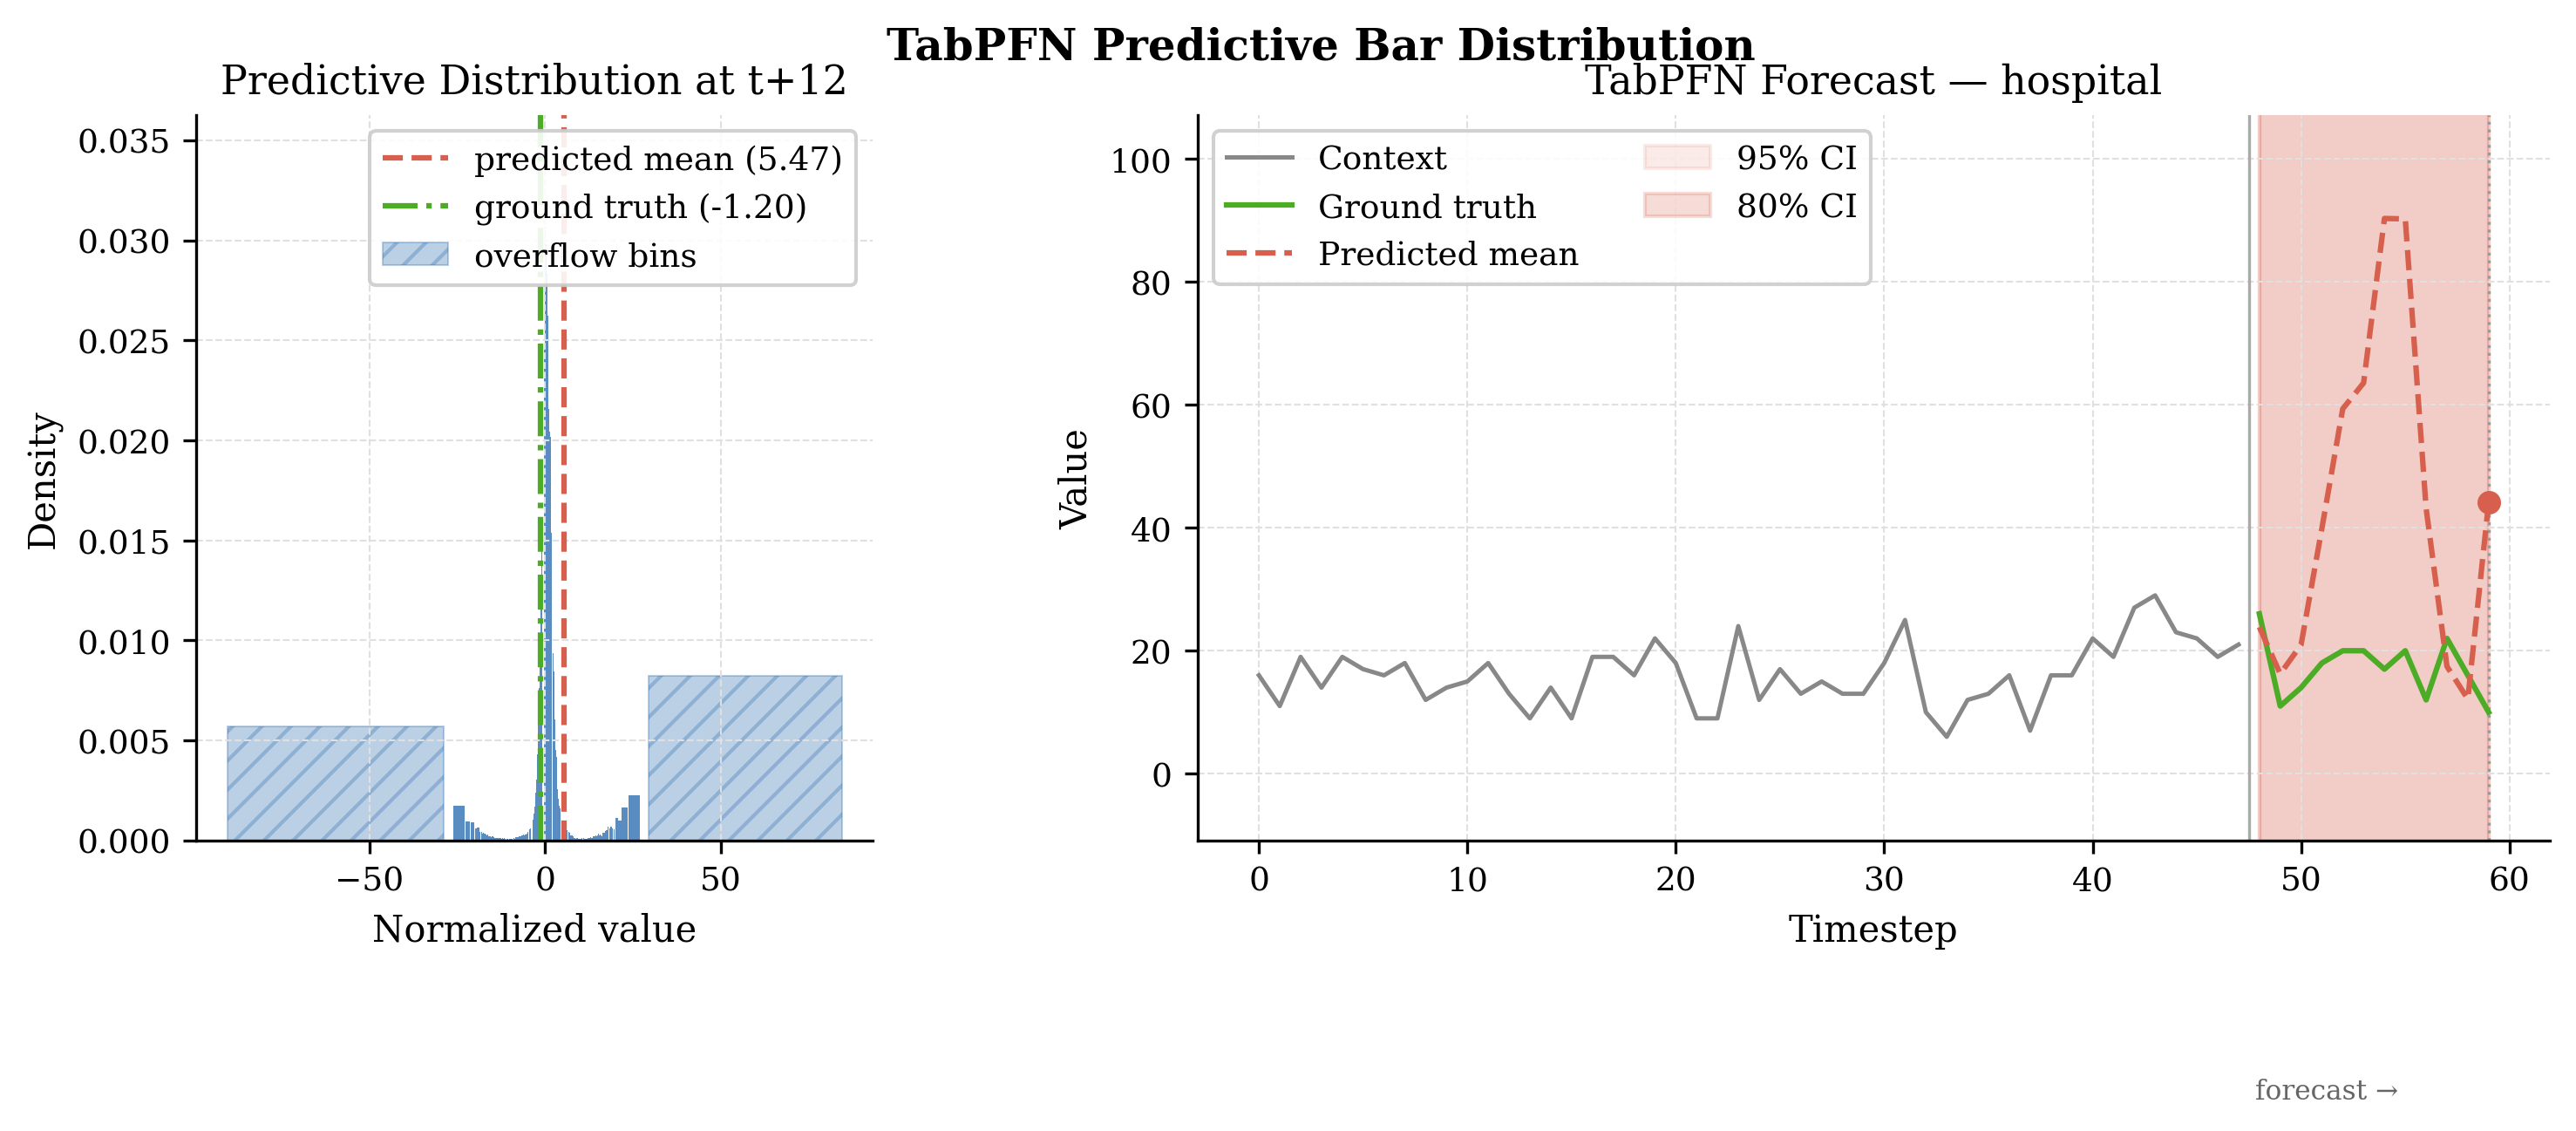
\includegraphics[width=0.8\textwidth]{pictures/bardist_hospital.png}
\caption{TabPFN Predictive Bar Distribution on the hospital dataset for the last predicted value. The boxes left and right in the bar distribution are cumulative densities for the given threshold.}
\label{fig:bardist_hospital}
\end{figure}
%classification point estimation?
\newline

TabPFN especially outperforms comparable models like CatBoost, Autogluon, etc.\ on small to medium-sized datasets with up to 10000 samples and 500 features \citep{hollmann2025accurate}.
This limitation results from the fact that the prior used during pretraining generated datasets only up to this size.\newline
Compared to gradient-boosted decision trees, a 3000x faster performance in regression and a 5140x faster performance in classification on a NVIDIA RTX 2080 Ti has been observed \ citep {hollmann2025accurate}. \newline
Another interesting detail researchers have discovered is that TabPFN works out of the box without any necessary hyperparameter tuning, especially in classification.
But even when using hyperparameter search, TabPFN showed remarkable and efficient results: After just 300s of hyperparameter tuning, TabPFN outperforms Autogluon, which was also hyperparameter-tuned, but for 4 hours.

While TabPFN achieves strong performance on tabular benchmarks, its generalization to other data modalities is not guaranteed.
In particular, its performance on time series data depends on how effectively temporal information is encoded into tabular features.
\subsection{TabPFN-TS}
\label{subsec:tabpfnts}
\citet{hoo2025tables} introduce TabPFN-TS: A model that combines TabPFN with lightweight feature engineering to enable both point and probabilistic forecasting.
Point forecasting predicts a single value, while probabilistic forecasting returns a distribution of quantiles.
As mentioned in \autoref{subsec:time_series_as_tabular}, \citet{hoo2025tables} split these data into the following features.
\subsubsection{Running Index}
The Running index is one feature that serves as an index for each observation in the time series to provide an effective way to track progression in time series.
The first Observation has a running index of 0, the next has a running index of 1, and so on.
Formally, this adds the following feature to $X$:
\[
\Phi_{index}(t) = t \in \mathbb{R}
\]
\subsubsection{Calendar Features}
To give TabPFN a better understanding of the temporal cycle that is used in our society, the timestamp data is encoded into eight cyclic calendar components.
These are: second of minute, minute of hour, hour of day, day of week, day of month, day of year, week of year, and month of year.
To encode these values into cyclic values, the sine and cosine functions are both separately applied to each calendar component.
Additionally, the current calendar year is also included as a non-cyclic component.
So each timestamp t is encoded in the following:
\[
\Phi_{cal}(t)=\left(cos\left(\frac{2 \pi t}{P_1}\right), sin\left(\frac{2 \pi t}{P_1}\right), …, cos\left(\frac{2 \pi t}{P_8}\right), sin\left(\frac{2 \pi t}{P_8}\right), year(t)\right) \in \mathbb{R}^{17}
\]
With ${P_{i}}^8_{i=1}$ being the periods of the calendar components.
\subsubsection{Automatic Season Features}
Most time series exhibit domain-specific cycles that cannot be captured by calendar features.
To also take these cycles into account, \citet{hoo2025tables} introduces an algorithm that extracts the top-k periodicities and encodes them as features.
At first, the series is detrended with the use of a simple least squares regression.
After that, to reduce spectral leakage and improve frequency resolution, a Hann window is applied, and the windowed signal is zero-padded by a factor of two.
Now, to extract the features, the real-valued Fourier transformation is calculated and the zero-frequency component, which corresponds to the mean value, is removed \citet{hoo2025tables}.
After that, the k largest spectral peaks by magnitude $f_1, …, f_k$ are selected, and the features are calculated as follows:
\[
\Phi_{auto}(t) = (cos(2\pi f_1 t), sin(2 \pi f_1 t), …, cos(2\pi f_k t), sin(2 \pi f_k t)) \in \mathbb{R}^{2k}
\]
\subsubsection{Time-varying Covariates (when available)}
Also, known time-varying covariates like holidays can be taken into account and are denoted as follows:
\[
z_{1:C+H} = [z_1, …, z_{C+H}]
\]
where $z_t \in \mathbb{R}^{D_{z}}$ represents $D_z$ external variables observed at time \textbf{t}
\newline
\
Each timestamp $x_t \in X=X_{train} \cup X_{test}$ is now defined as:
\[
x_t = \Phi_{index}(t) \oplus \Phi_{cal}(t) \oplus \Phi_{auto}(t) \oplus z_t \in \mathbb{R}^{18+2k+D_z}
\]

To avoid much slower inference, TabPFN-TS does not rely on lagged or auto-regressive features like moving averages or lag terms as comparable models do.
\newline
With the help of this encoding, TabPFNv2 is able to achieve state-of-the-art performance in covariate-informed forecasting and competitive accuracy in univariate time series forecasting.
To evaluate TabPFN-TS, the GIFT-EVAL benchmark has been used \citep{hoo2025tables}.
\newline
In this thesis, we will use the code of the featurization as well as the evaluation to implement our finetuning pipeline.\footnote{\url{https://github.com/PriorLabs/tabpfn-time-series}}
\subsection{Finetuning}
\subsubsection{Definition}
Fine-tuning is commonly used in deep learning to adapt pretrained foundation models to specific tasks.
\newline
Foundation models are typically pretrained on large and heterogeneous datasets to achieve strong performance across a wide range of tasks within a given domain.
To further improve performance on a specific real-world dataset, the model is finetuned by training on that dataset.
\newline
Specifically for TabPFN, which was trained on artificial data created from a prior, it is crucial for finetuning to use a real-world dataset \citep{rubachev2025finetuning}.

Finetuning can improve performance on specific datasets, but may also lead to overfitting or reduced generalization.
In particular, improvements are often dataset-specific and may not transfer to other tasks.
Training on multiple datasets introduces extra variability, which may benefit generalization but complicates optimization.
\subsubsection{Related Work}
\citet{rubachev2025finetuning} lists two main ways of finetuning methods popular with tabular foundation models.
The first one is full finetuning, in which all parameters are updated as in the pretraining process.
The other one is parameter-efficient finetuning (PEFT), which is often used for LLM adaptation, since they have a significantly larger amount of parameters (TabPFN ~7M vs GPT-3 ~175B)\citep{brown2020language, hollmann2025accurate}.
The authors also found that full finetuning, due to its similar approach for improved retrieval-based assessments, is the superior way of finetuning TabPFNv2.
For this reason, we will also only investigate full finetuning in this thesis.\newline
While finetuning on one dataset improves performance on this specific dataset, finetuning on many datasets at once, like \citet{Hollmann_2025} did, showed significant performance boosts in downstream tasks.
They used the original TabPFNv2 configuration that was pretrained on artificial data and used a diverse amount of datasets for improvements.
Furthermore, they called this method `continued pretraining’, which is contrary to our assumption for this thesis that finetuning solely relies on training on real-world datasets, while continued pretraining uses artificial datasets from a prior.

\subsection{Continued Pretraining}
\subsubsection{Definition}
As mentioned above, we define continued pretraining as further training a foundation model on a domain-specific prior with the goal of improving its performance.
\subsubsection{Related Work}
There has been limited work on continued pretraining with domain-specific priors. However, \citet{kolberg2025tabpfn} showed that continuing to pretrain TabPFNv2 on a similar modality (tabular data with high feature dimensionality and low sample count) leads to decreased performance on datasets that do not exhibit these characteristics.
This demonstrates that while continued pretraining can be beneficial, its effects are highly dependent on the alignment between the prior and the target data distribution, indicating that possible benefits have not yet been fully explored.
\newline



\chapter{Finetuning TabPFN-TS}
In this section we will thoroughly explore the potential benefits of finetuning.
First we will finetune on a single dataset and evaluate on the same dataset.
Then we will finetune on multiple datasets while evaluating on independent datasets we did not train on.
\label{chap:finetuning}
TabPFN-TS already showed remarkable results on the GIFT-Eval benchmark.
But as shown in Figure~\ref{fig:hospital_tabpfn_ts_pred}, it still struggles especially with noisy and non-periodic time series.
\begin{figure}[H]
    \centering
    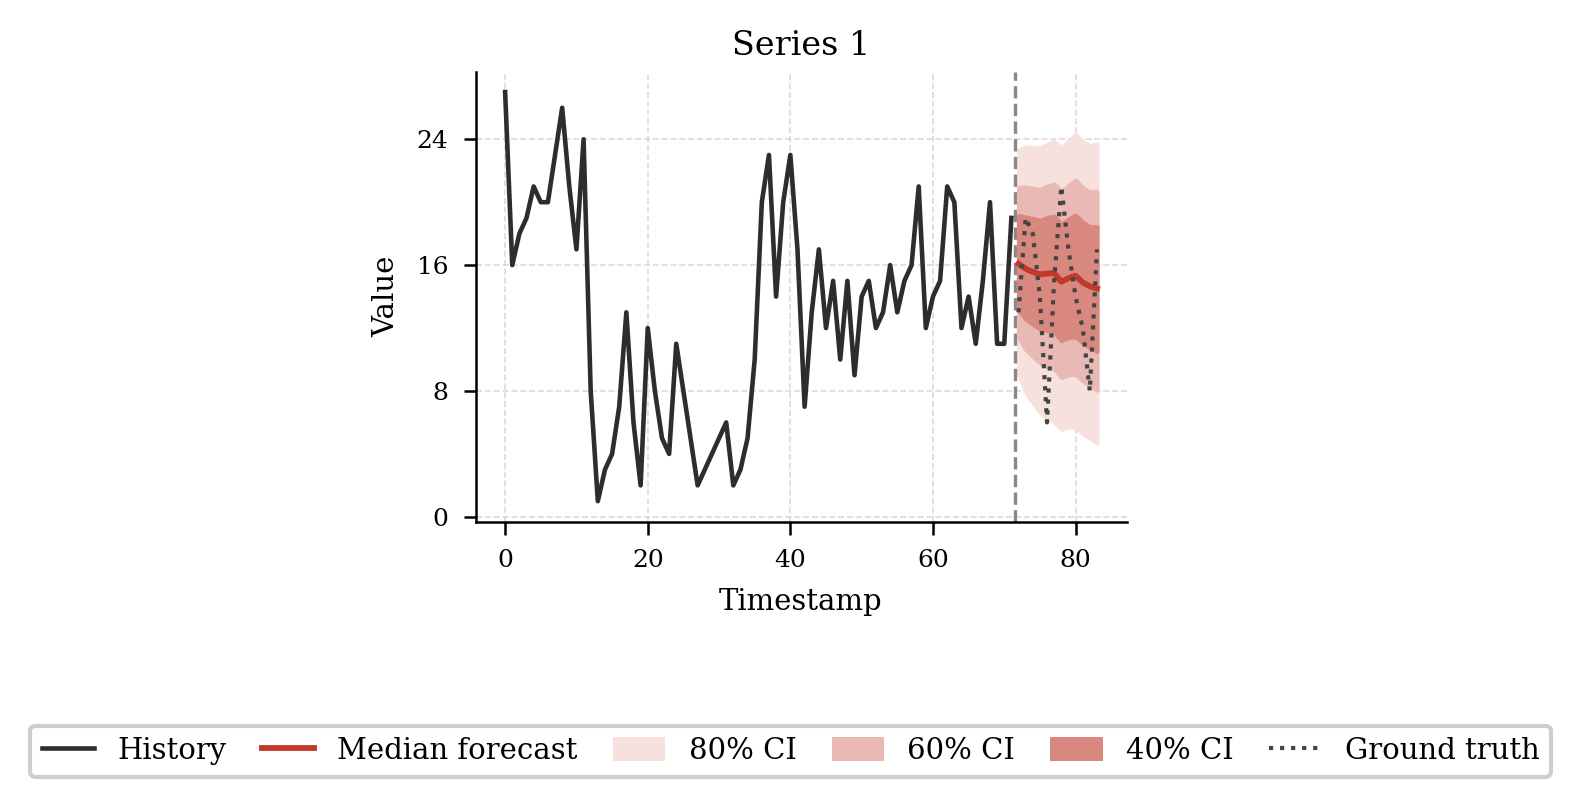
\includegraphics[width=0.8\textwidth]{pictures/hospital.png}
    \caption{Prediction by TabPFN-TS for the hospital dataset. As shown, the time series is very noisy and non-periodic; therefore, the forecast can only capture the trend.}
    \label{fig:hospital_tabpfn_ts_pred}
\end{figure}
In this section, we will further investigate the potential benefits of finetuning TabPFN-TS on the time-series datasets GIFT-Eval and autogluon/chronos-datasets.
For this endeavor, we will examine two methods of finetuning.
The first is finetuning on one dataset.
This will presumably enhance performance on the specific dataset we will train on and potentially other datasets that share some characteristics. %todo
The second method is finetuning on multiple datasets.
As \citet{Hollmann_2025} already showed, finetuning TabPFN across multiple datasets is equivalent to continuing pretraining, thereby enhancing performance across a wide range of datasets.
We will further investigate this by applying the method to time-series data.

\section{Experimental Setup}
%Zuerst daten vorbereitung(dataset_utils)
%daten pro training dataloader
%validation
%hyperparameter setup
%evaluation
For our experiments, we will use full supervised finetuning in which we update all parameters of the model.
This method has been proven to be the best way of finetuning TabPFN since the model is tolerant to full updates and has an insignificant amount of parameters \citep{tanna2026exploring}.

For the most part, the code that is used will be provided by Lennart Purucker's repository ``finetune tabpfn v2''.
Although most of the setup was completed with this, we still had to adjust the normalization of the training error to first make the script work for normal tabular data.
To let the script also finetune on time series data, we also had to make some adjustments in the data creation, batch creation, and validation.

\subsubsection{Data creation/transformation}
GIFT Eval contains 23 datasets, each comprising varying numbers of time series from different domains.
For each dataset, a forecast horizon is defined based on its frequency.
The frequency indicates how often observations are recorded, for example, daily, weekly, or monthly.\newline
Based on this and a predetermined number of sliding windows, training, validation, and test sets can be created for each time series in the dataset.
The test and validation splits have non-overlapping forecast targets to ensure that evaluation and validation are performed on unseen data not included during training.
This means that for a time series with $n$ values, a forecast horizon of $m$ and $w$ windows the training split contains the first $n-(m \cdot (w+1))$ observations, the validation split contains the first $n-(m \cdot w)$ observations and the test split contains all values with the last $(m \cdot w)$ being split into $w$ windows for benchmark evaluation.
This can be seen in the appendix in Figure~\ref{fig:gift_eval_split_us_births_m}.\newline
While only the test data is split into multiple sliding windows, we implemented that the training data is split into $w$ windows as well.
This will be done with the same method as the test split for each time series in a dataset, thus resulting in more training data.
\newline
To finetune TabPFN with time series data in the form of tabular data, we have to transform the data that is selected.
Every time series is transformed into 28 features containing the running index, calendar features, and automatic season features.
This will be done with the code provided by \citet{hoo2025tables} and as it was explained in the background.
\newline
Datasets with time series that do not have a constant length are not taken into account since they require padding to be useful for uniform batch creation.
Since TabPFN-TS was evaluated on GIFT-Eval using a maximum of 4096 points as context length, and for computational purposes, we also clipped all time series to this length.

GIFT-Eval supports three different prediction lengths for almost every dataset, e.g., \ short, medium, and long.
This is done by multiplying the original forecast horizon by different factors that are also based on the frequency of the dataset.
Note that we will only finetune using the short (so the original) forecast horizon, as extending it would exceed the available computational resources.

\subsubsection{Data loading/data selection/batch creation}

As explained in the Background part(here ref), instead of $(x, y)$, one sample consists of a set of n tuples with the form $(x_i, y_i)$.
So in training, one batch consists of $k$ samples, with $k$ also known as the batch size.

The selection of training and validation data fundamentally differs from that of tabular data.
For tabular data, before fine-tuning, one typically randomly selects nnn samples from the dataset and removes them to form the validation set.
Training samples are drawn in a similar way, but remain part of the original dataset.

For time series, the procedure is different.
Each dataset consists of multiple time series, and, as stated earlier, each time series is divided into training, validation, and test splits.

To create a validation set of $k$ predictions, $k$ time series are randomly selected, and their validation splits are used.
After that, we validate every $n$ steps and take the mean of all validation losses of each validation time series.
This validation loss is also used for early stopping, which we configured with a minimum patience of 100 and a maximum patience of 200.

To construct a training batch, one window is randomly sampled from a randomly chosen time series in the current dataset.
This process is repeated kkk times to create a batch of kkk training samples for one epoch.
The same sampling procedure is repeated in every epoch.

\subsubsection{Hyperparameters}
Additionally, to the standard hyperparameters such as batch size and learning rate, we also use a regularizer for the distance to the L2-Starting Point (L2-SP) \citep{xuhong2018explicit}.
Instead of a normal L2 distance, we penalize large deviations from the initial pretrained weights of the model $w^0$.
It is calculated via
\[
    \Omega(w)= \frac{\alpha}{2} \lVert w - w^0 \rVert
\]
where $\alpha$ is the regularization parameter setting the strength of the penalty, thus representing a hyperparameter.
\citet{Hollmann_2025} used it for their continued pretraining, and we wanted to see whether it also improves performance in our experiments

Instead of doing a hyperparameter search first to determine which hyperparameters perform best, we finetune TabPFN 54 times on one dataset for each different hyperparameter configuration.
We use batch sizes 2, 4, 8, 16, 32, and 64 as well as learning rates 0.0005, 0.00005, and 0.000005.
As $\alpha$ for the L2-SP Norm, we use 0, 0.003, and 0.0002.

After that, we take the 5 finetuning checkpoints with the best validation loss and evaluate on the GIFT-Eval evaluation.

\subsubsection{Evaluation}
For evaluation, we use the script provided by TabPFN-TS and only evaluate on short forecast horizons.
Note that we were not able to reproduce all benchmark results that are currently submitted in GIFT-Eval, so before finetuning, we evaluate every dataset on the base checkpoint and take it as a reference.
For the base checkpoint, we use the \textit{tabpfn-v2-regressor-2noar4o2} checkpoint, which was also used in \citet{hoo2025tables}.
To compare the evaluation results, we observe the Mean Absolute Scaled Error(MASE) and take the percentage difference compared to the original checkpoint, and average it for the five finetuning checkpoints.
If this value is negative, we conclude an improvement.
If it is positive, we conclude a worsening.
\section{Results}
This section will present the results of our finetuning experiments while not interpreting them. %TODO
\subsection{Finetuning on one Dataset}
\label{subsec:singlefinetuning}
For finetuning on one dataset, we, as the name suggests, only used data from one dataset.
Since many datasets from GIFT-Eval come with different observation frequencies, we use only the data from one frequency from one dataset, as it was divided in GIFT-Eval.
With this method, we were able to train TabPFN on 33 different datasets with different metadata like context length, time series amount, or forecast horizon.
After completing this procedure, we now have 54 checkpoints for each of the 33 datasets.
This is due to our method of evaluating 54 different configurations for hyperparameter tuning.

%TODO
We report the training summary in Figure~\ref{}, showing that validation loss has improved on all but two datasets.
By looking at each training summary, we can  see that on all except for two datasets, the validation loss improved in at least one of the checkpoints for each dataset.
The two datasets that did not improve regarding the validation loss are jena\_weather with frequency 10T and ett1 with frequency D, both of which are multivariate datasets with 20 and 7 varieties.

%To evaluate whether the fine-tuning process improved or degraded the performance of TabPFN-TS on our dataset, we rank all 54 checkpoints for each dataset according to their validation loss and select the top five.
%This will result in five lists of different error metrics for each dataset, from which we will select the MASE as we mentioned earlier, and the percentage difference to its original checkpoint.
We further evaluated the Top-5 configurations according to validation loss and compare the percentage difference in MASE to the original checkpoint.


As you can see in Figure~\ref{tab:eval_score_single_finetune} is that only 14 finetuning runs led to an improved average performance for every dataset.

Another thing that can be seen in Figure~\ref{tab:eval_score_single_finetune} in the appendix, the order of the checkpoints that were selected via the validation loss is not the same as the order in which they are in evaluation performance.
Not only that, but it also does not always indicate an improvement on the benchmark regarding the dataset if the validation loss itself improved.

An example can be seen in Figure~\ref{fig:eval_M_DENSE_H} by looking at the five evaluated checkpoints of the dataset M\_DENSE with hourly frequency.
\begin{figure}[H]
    \centering
    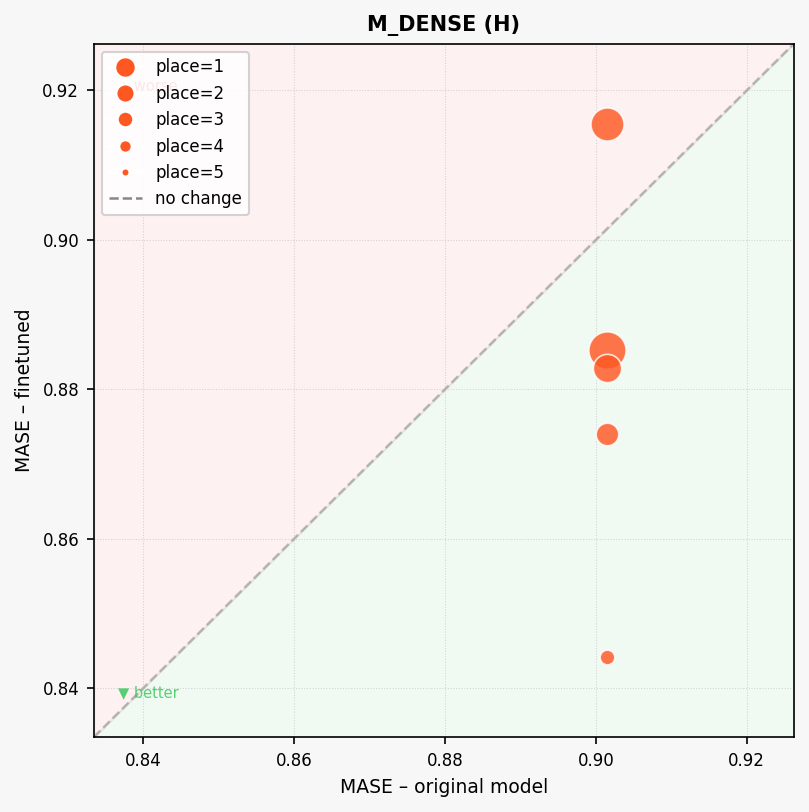
\includegraphics[scale=0.5]{pictures/eval_M_DENSE_H.png}
    \caption{Evaluation results of finetuning with M\_DENSE dataset with hourly frequency. The picture shows an improvement and worsening of the top five checkpoints. As already mentioned, they are not in order regarding the validation loss.}
    \label{fig:eval_M_DENSE_H}
\end{figure}
% TODO prozentual Plot der Verbesserung zeigen Balkendiagramm


\begin{figure}[H]
    \centering

    \begin{subfigure}[t]{0.48\textwidth}
        \centering
        
\includegraphics[width=\linewidth]{pictures/plot1_score_series.pdf}
        \caption{Score Series}
        \label{fig:plot1_score_series}
    \end{subfigure}
    \hfill
    \begin{subfigure}[t]{0.48\textwidth}
        \centering
        
\includegraphics[width=\linewidth]{pictures/plot2_context_vs_series.pdf}
        \caption{Context vs Series}
        \label{fig:plot2_context_vs_series}
    \end{subfigure}

    \caption{Listing of both plots regarding the context length and time series amount. Green marks an improvement, while red indicates performance degradation. }
    \label{fig:combined_plots}
\end{figure}
In Figure~\ref{fig:plot1_score_series} shows the relationship between the total number of observations per dataset and the MASE difference.
For datasets with more than 100,000 observations, the MASE difference is predominantly negative.

Figure~\ref{fig:plot2_context_vs_series} illustrates that datasets with both high context length and many time series are predominantly associated with negative MASE differences.
%If there is a notable amount of time series and a notable amount of context finetuning was successful and improved performance.
Datasets with only one of these characteristics are more frequently associated with positive MASE differences.
This can be observed particularly in datasets containing only a single time series, which, with few exceptions, perform worse than before fine-tuning.

\subsection{Finetuning on multiple Datasets}
\label{subsec:multifinetuning}
Next, we fine-tune TabPFN on multiple time series datasets simultaneously.
This is done by first selecting a handful of datasets we want to use for training, and then for every epoch randomly selecting one dataset we want to build the batch from.
For the next epoch, data from another dataset will be drawn.

Validation is done by validating on every dataset we also use for training, normalizing the error, and adding it together to get a combined validation error for a large number of datasets.

Instead of finetuning TabPFN on a large amount and variety of datasets, we decided to split the datasets into three categories with respect to different context lengths, motivated by \citet{Hollmann_2025}.
They concluded that longer context resulted in better results, and we wanted to validate these results.
We defined the threshold for each category as follows: Small $\rightarrow$ 0-250, Medium $\rightarrow$ 250-1000, Large $\rightarrow$ 1000-Inf.
Note that all time series with a context length greater than 4096 were truncated, as 4096 is the largest context length considered during training, following \citet{hoo2025tables}.

We evaluate our finetuned models in three settings:
The unseen test sets of the datasets it was trained on, unseen datasets from the same category, and unseen datasets from different categories.
%For independent evaluation, we are limited to datasets we did not finetune with.
%This limits most of the categories to only a few datasets.
%So for our plan, we also evaluate on datasets we trained with and datasets from other categories to check if performance improves across the board.
%Both of these are marked in the plots.
\subsubsection{Small Context Length}
For datasets that have a small context length (0-250 observations per time series), we selected the following for training:
\begin{table}[H]
\centering
\begin{tabular}{lrr}
\hline
Dataset & Context Length & Num Series \\
\hline
ett1/W & 103 & 1 \\
hospital & 84 & 767 \\
electricity/W & 208 & 370 \\
covid\_deaths & 212 & 266 \\
ett2/W & 103 & 1 \\
\hline
\end{tabular}
\caption{}
\label{tab:datasets}
\end{table}
Since there are few datasets with a short context length, we were only able to independently evaluate the checkpoints on one dataset.
\begin{table}[H]
\centering
\begin{tabular}{lrr}
\hline
Dataset & Context Length & Num Series \\
\hline
solar/W & 52 & 137 \\
\hline
\end{tabular}
\caption{}
\label{tab:solar_w}
\end{table}
Additionally to this, and as stated above, we will also evaluate on the datasets we trained on, as well as two datasets that are from the medium and big categories.
These two datasets are the following:
\begin{table}[H]
\centering
\begin{tabular}{lrrr}
\hline
Dataset & Context Length & Num Series & Category \\
\hline
LOOP\_SEATTLE/D & 365 & 323 & Medium \\
M\_DENSE/H & 17520 & 30 & Large \\
\hline
\end{tabular}
\caption{}
\label{tab:selected_datasets}
\end{table}
% first run
% list dataset we finetuned with
% list dataset we evaluated with and results
% list datasets we also trained with
\begin{figure}[H]
    \centering
    
\includegraphics[scale=0.7]{pictures/multi_short/mase_mean_delta_plot.png}
    \caption{Horizontal diverging bar chart for multi-dataset fine-tuning with short context length. Lower is better.}
    \label{fig:multi_short_mase_mean_delta_plot}
\end{figure}
\begin{table}[H]
\centering
\resizebox{\textwidth}{!}{
\begin{tabular}{l l c r r r r r r r r r c}
\hline
dataset & context & trained & num & ckpt1 & ckpt2 & ckpt3 & ckpt4 & ckpt5 & mean & min & max & imp \\
\hline
m\_dense/H      & big    & F & 1 & 18.25 & 36.51 & 15.43 & 2.53 & 7.19 & 15.98 & 2.53 & 36.51 & F \\
loop\_seattle/D & medium & F & 1 & 5.87 & 10.17 & 4.17 & \textbf{-1.35} & 2.55 & 4.28 & -1.35 & 10.17 & F \\
solar/W        & short  & F & 1 & \textbf{-1.27} & -0.07 & 2.93 & 3.76 & 44.53 & 9.98 & -1.27 & 44.53 & F \\
hospital/M     & short  & T & 1 & 7.12 & 0.92 & 5.24 & \textbf{-0.46} & 0.56 & 2.68 & -0.46 & 7.12 & F \\
electricity/W  & short  & T & 1 & 4.44 & 8.86 & 6.01 & \textbf{-2.60} & 4.09 & 4.16 & -2.60 & 8.86 & F \\
ett1/W       & short  & T & 7 & -11.15 & -1.99 & \textbf{-13.80} & -9.13 & -11.30 & -9.47 & -13.80 & -1.99 & T \\
covid\_deaths/D & short  & T & 1 & 23.00 & 68.43 & 5.89 & 16.77 & 19.65 & 26.75 & 5.89 & 68.43 & F \\
ett2/W         & short  & T & 7 & 97.35 & 81.49 & 45.00 & 44.82 & 97.17 & 73.16 & 44.82 & 97.35 & F \\
\hline
\end{tabular}
}
\caption{Results of the five checkpoints for multi-dataset fine-tuning with short context length and their percentage difference to the original checkpoint. If a checkpoint resulted in an improvement (negative value), it is shown in bold when it also corresponds to the smallest value.}
\label{tab:multi_short_wide_results}
\end{table}
We report results in Figure~\ref{fig:multi_short_mase_mean_delta_plot} and Table~\ref{tab:multi_short_wide_results}.
As the graph depicts, the mean performance of all 5 best checkpoints performed significantly worse than the original checkpoint on almost all datasets.
The MASE not only worsened on the designated evaluation dataset but also worsened on the dataset we trained with, as well as the two datasets that came from a different category.
The only exception is ett1/W, where we can see a small average improvement of 1,99 percent.
This behavior can be observed across all top 5 checkpoints.
So, all five checkpoints performed almost the same.

\subsubsection{Medium Context Length}
For medium-sized datasets, there was more data available, thus more data to independently evaluate TabPFN on.
But first, for training, we chose the following datasets with their context length and time series amount.
\begin{table}[H]
\centering
\begin{tabular}{lrr}
\hline
Dataset & Context Length & Time Series Length \\
\hline
ett2/D & 725 & 1 \\
sz\_taxi/H & 744 & 156 \\
us\_births/M & 240 & 1 \\
solar/D & 365 & 137 \\
ett1/D & 725 & 1 \\
m\_dense/D & 730 & 30 \\
\hline
\end{tabular}
\caption{}
\label{tab:ctx_ts}
\end{table}
As mentioned before, independent evaluation datasets (so datasets we did not train with) are not as scarce as they were in the short context length category, so we had more datasets to evaluate on.
For evaluation, we chose the following:
\begin{table}[H]
\centering
\begin{tabular}{lrr}
\hline
Dataset & Context Length & Time Series Length \\
\hline
bitbrains\_rnd/H/short & 720 & 500 \\
loop\_seattle/D & 365 & 323 \\
saugeenday/M & 780 & 1 \\
hierarchical\_sales/W & 260 & 118 \\
\hline
\end{tabular}
\caption{}
\label{tab:ctx_ts_2}
\end{table}
And to check whether performance also improved on datasets that were not even in the category, we chose the following two:
\begin{table}[H]
\centering
\begin{tabular}{lrrr}
\hline
Dataset & Context Length & Time Series Length & Category \\
\hline
sz\_taxi/15T & 2976 & 156 & Large\\
covid\_deaths/D & 212 & 266 & Small\\
\hline
\end{tabular}
\caption{}
\label{tab:ctx_ts_3}
\end{table}

%TODO Plots: Mean plot
%TODO table of evaluation
%TODO table of hp
After training, we got the following results over all evaluated datasets
\begin{figure}[H]
    \centering
    
\includegraphics[scale=0.7]{pictures/multi_medium/mase_mean_delta_plot.png}
    \caption{Horizontal diverging bar chart of multi-dataset fine-tuning with short context length. Lower is better.}
    \label{fig:multi_medium_mase_mean_delta_plot}
\end{figure}
The results are completely different from those of short context finetuning.
What is immediately apparent is that, on average across all five checkpoints, 8 out of 12 datasets show a performance improvement.
On all datasets, which we only used for evaluation, TabPFN performed better than the original checkpoint.
Contrary to that, 3 out of 6 datasets we trained TabPFN with experienced a performance loss in the evaluation.

\begin{table}[H]
\centering
\resizebox{\textwidth}{!}{
\begin{tabular}{l l c r r r r r r r r r c}
\hline
dataset & context & trained & num & ckpt1 & ckpt2 & ckpt3 & ckpt4 & ckpt5 & mean & min & max & imp \\
\hline
covid\_deaths/D        & short  & F & 1 & 7.91 & 9.15 & 14.74 & 18.53 & 27.55 & 15.58 & 7.91 & 27.55 & F \\
sz\_taxi/15T           & big    & F & 1 & \textbf{-0.83} & -0.71 & -0.53 & 0.69 & 0.31 & -0.22 & -0.83 & 0.69 & T \\
bitbrains\_rnd/H       & medium & F & 2 & -0.93 & -0.92 & -1.73 & \textbf{-3.00} & -1.91 & -1.70 & -3.00 & -0.92 & T \\
loop\_seattle/D        & medium & F & 1 & \textbf{-2.83} & -2.52 & -1.91 & -0.38 & -0.08 & -1.54 & -2.83 & -0.08 & T \\
saugeen/M             & medium & F & 1 & 0.60 & -0.50 & 1.58 & -0.43 & \textbf{-3.49} & -0.45 & -3.49 & 1.58 & T \\
hierarchical\_sales/W  & medium & F & 1 & \textbf{-1.16} & -0.92 & -0.55 & 1.02 & 0.13 & -0.30 & -1.16 & 1.02 & T \\
ett2/D                & medium & T & 7 & -34.85 & \textbf{-35.17} & -34.10 & -22.96 & -29.19 & -31.26 & -35.17 & -22.96 & T \\
sz\_taxi/H             & medium & T & 1 & -1.89 & \textbf{-1.90} & -1.57 & -0.18 & 0.36 & -1.04 & -1.90 & 0.36 & T \\
us\_births/M           & medium & T & 1 & -5.32 & \textbf{-14.80} & -7.64 & 0.94 & 24.62 & -0.44 & -14.80 & 24.62 & T \\
solar/D               & medium & T & 1 & 1.01 & 1.02 & \textbf{-2.72} & 0.57 & 0.46 & 0.07 & -2.72 & 1.02 & F \\
ett1/D                & medium & T & 7 & 1.27 & 0.17 & 6.21 & 1.18 & 2.23 & 2.21 & 0.17 & 6.21 & F \\
m\_dense/D             & medium & T & 1 & \textbf{-0.52} & 0.00 & 1.65 & 4.04 & 5.94 & 2.22 & -0.52 & 5.94 & F \\
\hline
\end{tabular}
}
\caption{Results of the five checkpoints for multi-dataset fine-tuning with medium context length. If a checkpoint resulted in an improvement (negative value), it is shown in bold when it also corresponds to the smallest value.}
\label{tab:medium_context_wide_results}
\end{table}
By looking at~\ref{tab:medium_context_wide_results}, we can see that checkpoint 2 performs best out of the 5 checkpoints we evaluated on.
Checkpoints 4 and 5 performed on average worse and only improved performance on 6 and 7 datasets.
The dataset of the short category performed worse on all checkpoints.

\begin{table}[H]
\centering
\resizebox{\textwidth}{!}{
\begin{tabular}{l r r r r r r r r r r r l r r}
\hline
ckpt & Time & LR & BS & L2-SP & WD & TimeTot & InitLoss & BestLoss & LastLoss & Steps & BestStep & ES Reason & t/step & Util \\
\hline
ckpt\_1 & 2400 & 5e-05 & 32 & 0.0 & 0.0 & 531.13 & 0.3873 & 0.3327 & 0.3361 & 470 & 259 & AdaptiveES & 1.13 & 98.78 \\
ckpt\_2 & 2400 & 5e-05 & 32 & 0.0001 & 0.0 & 513.75 & 0.3873 & 0.3330 & 0.3409 & 450 & 249 & AdaptiveES & 1.14 & 98.84 \\
ckpt\_3 & 2400 & 5e-05 & 8 & 0.0001 & 0.0 & 267.59 & 0.3873 & 0.3352 & 0.3511 & 520 & 309 & AdaptiveES & 0.51 & 88.65 \\
ckpt\_4 & 2400 & 0.0005 & 32 & 0.0001 & 0.0 & 564.65 & 0.3873 & 0.3358 & 0.3632 & 500 & 299 & AdaptiveES & 1.13 & 98.67 \\
ckpt\_5 & 2400 & 0.0005 & 16 & 0.0015 & 0.0 & 343.30 & 0.3873 & 0.3360 & 0.3412 & 490 & 289 & AdaptiveES & 0.70 & 96.84 \\
\hline
\end{tabular}
}
\caption{Training Runs mit verschiedenen Checkpoints}
\label{tab:medium_context_training_ckpts}
\end{table}

The hyperparameters are also an interesting topic to look at.
\ref{tab:medium_context_training_ckpts} showed that 4 out of 5 checkpoints used the L2-SP lambda also used in \ref{realtabpfn}.
Checkpoints 4 and 5 used a learning rate of 0.0005, contrary to checkpoints 1-3, which used 0.00005.

% im mean wird es auf 8 besser und auf 4 schlechter
% auf 3 datensets auf denen auch trainiert wurde wurde es schlechter
% auf datensets auf denen nicht trainiert wurde und nur evaluiert wurde und auch medium length haben wurde es nur besser bzw ziemlich gleich
%
% checkpoint 2 performed am besten über alle datensets
% checkpoints 4 und 5 performen schlechter als der durchschnitt
% auf short viel verschlechtert und auf big context length nicht signifikant verbessert aber auch nicht verschlechtert
% bei hyperparametern sind l2 sp lambda in 4/5 checkpoints drin
% da ckpt 4 und 5 schlechter performen und lr 0.0005 haben schlechter im vergleich zu 0.00005
% TODO prozentual plot der verbesserung zeigen balken diagramm
%
\subsubsection{Big Context Length}
% list dataset we finetuned with
% list the dataset we evaluated with
% list datasets we also trained with
The last multi-finetuning category is of the big context length category.
All datasets in this category consist of time series with a context length of at least 1000 observations.
So, for training, we chose the following ones.
\begin{table}[H]
\centering
\begin{tabular}{lrr}
\hline
Dataset & Context Length & Time Series Length \\
\hline
hierarchical\_sales/D & 1825 & 118 \\
electricity/D & 1461 & 370 \\
sz\_taxi/15T & 2976 & 156 \\
m\_dense/H & 17520 & 30 \\
\hline
\end{tabular}
\caption{}
\label{tab:ctx_ts_4}
\end{table}
As well as the medium category, the large context length category also provides more datasets than the short context length category, so we will have more datasets to independently evaluate on.
For evaluation, we take:
\begin{table}[H]
\centering
\begin{tabular}{lrr}
\hline
Dataset & Context Length & Time Series Length \\
\hline
saugeenday/D/short & 23741 & 1 \\
us\_births/D/short & 7305 & 1 \\
ett1/15T & 69680 & 1 \\
ett1/H & 17420 & 1 \\
ett2/H & 17420 & 1 \\
ett2/15T & 69680 & 1 \\
\hline
\end{tabular}
\caption{}
\label{tab:ctx_ts_5}
\end{table}
To evaluate whether the trained checkpoints also improved on datasets that are not in the same category (so they have fewer observations than 1000), we also evaluate on these two datasets.
\begin{table}[H]
\centering
\begin{tabular}{lrrr}
\hline
Dataset & Context Length & Time Series Length & Category \\
\hline
covid\_deaths/D & 212 & 266 & Small\\
loop\_seattle/D & 365 & 323 & Medium\\
\hline
\end{tabular}
\caption{}
\label{tab:ctx_ts_6}
\end{table}
%TODO Plots: Mean plot
%TODO table of evaluation
%TODO table of hp
Our evaluation emitted the following results:
\begin{figure}[H]
    \centering
    
\includegraphics[scale=0.7]{pictures/multi_big/mase_mean_delta_plot.png}
    \caption{Horizontal diverging bar chart of multi-dataset fine-tuning with short context length. Lower is better.}
    \label{fig:multi_medium_mase_mean_delta_plot}
\end{figure}
8 out of 12 datasets show improved average results over all checkpoints compared to the original checkpoint.
But on most of these datasets, the improvement is not as significant as that of others.
Looking at the evaluation datasets, we see that 4 out of 6 datasets show an improvement compared to the original.

The short dataset also became worse than the original.

\begin{table}[H]
\centering
\resizebox{\textwidth}{!}{
\begin{tabular}{l l c r r r r r r r r r c}
\hline
dataset & context & trained & num & ckpt1 & ckpt2 & ckpt3 & ckpt4 & ckpt5 & mean & min & max & imp \\
\hline
covid\_deaths/D       & short & F & 1 & 23.56 & 77.34 & 49.68 & 49.19 & 44.23 & 48.80 & 23.56 & 77.34 & F \\
loop\_seattle/D       & medium& F & 1 & -1.92 & -1.96 & \textbf{-2.80} & -2.62 & -2.07 & -2.27 & -2.80 & -1.92 & T \\
ett1/15T             & big   & F & 7 & -2.98 & -5.00 & \textbf{-7.94} & -7.19 & -5.88 & -5.80 & -7.94 & -2.98 & T \\
ett1/H               & big   & F & 7 & -0.03 & \textbf{-4.94} & -2.68 & -2.64 & -2.60 & -2.58 & -4.94 & -0.03 & T \\
saugeen/D            & big   & F & 1 & 1.82 & -2.55 & \textbf{-4.33} & -2.01 & 2.08 & -1.00 & -4.33 & 2.08 & T \\
ett2/H               & big   & F & 7 & -1.79 & \textbf{-4.05} & -0.47 & -0.81 & 2.61 & -0.90 & -4.05 & 2.61 & T \\
ett2/15T             & big   & F & 7 & 1.77 & -0.42 & \textbf{-1.67} & -1.36 & 0.20 & -0.30 & -1.67 & 1.77 & T \\
us\_births/D          & big   & F & 1 & 34.64 & 20.01 & -- & 20.01 & 19.44 & 23.53 & 19.44 & 34.64 & F \\
hierarchical\_sales/D & big   & T & 1 & -1.35 & -1.44 & -0.33 & -0.30 & \textbf{-1.62} & -1.01 & -1.62 & -0.30 & T \\
electricity/D        & big   & T & 1 & 1.65 & \textbf{-3.18} & -0.77 & -0.63 & -0.45 & -0.68 & -3.18 & 1.65 & T \\
sz\_taxi/15T          & big   & T & 1 & 0.05 & \textbf{-0.27} & 0.20 & 0.22 & 0.05 & 0.05 & -0.27 & 0.22 & F \\
m\_dense/H            & big   & T & 1 & 1.01 & -1.63 & 2.12 & 2.10 & \textbf{-2.21} & 0.28 & -2.21 & 2.12 & F \\
\hline
\end{tabular}
}
\caption{Results of the five checkpoints for multi-dataset fine-tuning with large context length. If a checkpoint resulted in an improvement (negative value), it is shown in bold when it also corresponds to the smallest value.}
\label{tab:wide_results_3}
\end{table}
By looking at~\ref{tab:wide_results_3}, we can see that checkpoint 2 performed best out of all datasets and checkpoint 1 performed worst.
% 4/6 individuellen Datensets wurde es besser bzw. hat sich nicht verschlechtert
% 7 Datensets wurden besser. Davon 2, auf denen auch trainiert wurde.


% TODO prozentual Plot der Verbesserung zeigen Balkendiagramm

\section{Discussion}
The first research question we developed in the expose is ``Can we finetune TabPFN for time series with time-series data (and does it improve the performance)?''.
Our results that we got by finetuning TabPFN-TS on all 33 datasets of GIFT-Eval indicate that this question can be answered with a yes.
But it is dependent on the structure and features of the dataset.

% Validation Loss nicht richtige Order bzw. Indikator, dass Validierung besser ist
We first examine the significance of the validation loss for improved evaluation results.
As mentioned in the results section, we saw few to no correlations between the order of checkpoints regarding the validation loss and the order of them regarding the evaluation loss.
For example, in Figure~\ref{fig:eval_M_DENSE_H} we saw that the fifth checkpoint outperforms all of the other four checkpoints that were selected in order of validation loss.
Firstly, this is likely because the validation loss is MSE, whereas for evaluation we use the MASE.
Secondly, it is also because the data most likely overfits the validation data.
Datasets with one time series often halve their validation loss but show worsening in evaluation (e.g., see results on datasets). %TODO

By looking at Figure~\ref{fig:plot1_score_series}, we saw that the number of observations in one dataset highly correlates with the improvement we get from finetuning.
If a dataset has more than 100 thousand total observations, finetuning will most likely succeed by improving the evaluation loss.
%Hier nochmal theoretischen Teil mit Paper
Results in Figure~\ref{fig:plot2_context_vs_series}, further confirm this trend showing that finetuning on large context sizes and large amount of time series often improve performance.%where one can see a correlation between a large amount of context per series and a large amount of time series in a dataset, and an improved performance.
This now not only indicates that the number of observations contributes to an improved finetuning run, but also the structure of the dataset itself by providing multiple time series with a certain amount of datapoints.
\newline
Time series datasets differ from standard tabular datasets in that the tables within a dataset stem from the same domain and share a common distribution.
A longer individual time series does not necessarily lead to better fine-tuning (with some exceptions).
However, providing multiple time series (and thus multiple tables) appears to benefit fine-tuning.
An example is weather forecasting: having observations from multiple weather stations within the same city provides more information, as different stations exhibit variation in their measurements while still following nearly the same underlying distribution.

%failure cases
There are some exceptions to this.
We identified two tasks characteristics that make finetuning harder: Noisy datasets and intermittent data.
If we take a look at the hospital dataset that we also used as an example in Figure~\ref{fig:hospital_tabpfn_ts_pred}, we can see a small downwards trend but not periodicities.
This characteristic is typical for a noisy dataset: Random fluctuations that make it difficult for any forecasting model to predict.
This has been observed in prior work reporting that time series forecasting models have problems predicting on noisy datasets, as they were mostly trained on well-composed time series and have a hard time finding a schema in these data \citep{gupta2025evaluating}.
\newline
% TODO Soll ich überhaupt drinlassen?
Other datasets show other characteristics that make it hard for TabPFN to train on.
Looking at~\ref{bizitop_TODO}, we can see that in this dataset, a signal emerges periodically, but not in the same amplitude every time.
Between those signals, the values of the time series are constantly at or near zero.
This type of data is called intermittent data.
\citet{KieferGrimmBaueretal_2021} talked about this issue and came to the conclusion that deep learning approaches perform well, but still struggle to fully adapt to this type of data.
This could be a cause for TabPFN to not be able to finetune well on this type of data, as it was not able to find a good structure in this data.
%- schlecht zu quantifizieren aber Datensätze mit Time Series die sehr "noisy"(also nicht vorausschaubar) sind funktionieren nicht so gut weil TabPFN kein Schema finden kann (hier vielleicht https://arxiv.org/abs/2501.00889 aber das Paper sieht bisschen komisch aus)
%- Wenn Signal nur sehr selten kommt und dazwischen das Signal "konstant" ist, lernt es auch schlecht (intermittent Daten) https://link.springer.com/article/10.1007/s10479-023-05447-7
%hier erklären
% especially datasets with challenging structure were bad at finetuning
Overall, these results show that finetuning TabPFN-TS on real-world time series data can improve forecasting performance, but only under certain conditions.
In particular, success depends strongly on dataset size, structure, and signal quality, while noisy or intermittent datasets remain challenging.

\iffalse
- immer mit Research-Frage anfangen
- Fine-tuning on one dataset teuer weil viele Hyperparameter und nicht die eine Hyperparameter Config gefunden wurde
- dass der Validation Loss bei allen runtergeht aber die Evaluation nicht immer klappt lässt sich mit Overfitting auf den Validation Sets erklären
- Das sieht man vor allen Dingen bei den Datensets, die nur eine Zeitreihe haben -> Validation Loss wird manchmal halbiert, aber Evaluation viel schlechter
- Wenn das Signal nur sehr selten kommt und dazwischen das Signal "konstant" ist, lernt es auch schlecht (intermittent Daten) https://link.springer.com/article/10.1007/s10479-023-05447-7
- conclusion -> Es geht aber es gibt limitations durch Charakteristiken von Datensets und ihren Time Series
\fi

The question we investigate in our multi-dataset fine-tuning experiments is:
"Can we further improve performance by finetuning on multiple datasets similar to RealTabPFN \citep{Hollmann_2025}?"
This question can be answered with a yes, although not every category we established equally helped train the model to perform better on our evaluation datasets.
In the upcoming section, we will assess the different categories and finally compare them to single finetuning.

Finetuning with the small context lengths category only led to worsening.
This can be observed not only in our evaluation datasets but also in almost all datasets we trained on, including those from the multi and big categories.
This result goes hand in hand with the results also obtained by \citep{Hollmann_2025}.
A possible reason for this is the lack of information we have due to the smaller context.
TabPFN is not able to identify underlying structures in the data, thus generating a noisier gradient.
\newline
Another possibility is the differences regarding the characteristics of the time series.
Given that the context length is already small, it is also problematic that this occurs.

In contrast, the medium category achieved the best results out of all three methods.
Based on the five checkpoints, TabPFN-TS improved on average on nearly all evaluation datasets.
This is likely due to a larger number of datasets in this category, as well as more equally distributed characteristics that make it easier for TabPFN to learn with.
\newline
This performance does not distribute equally across all five checkpoints; it applies only to the first two.
An important factor that separates these two checkpoints from the other lower-performing ones is the learning rate.
The first two trained with a learning rate of 0.00005, while the other three trained with a learning rate of 0.0005.
This suggests that a more conservative approach with lighter updates suits TabPFN finetuning better in this context length setting.
% TODO average context length

For the training run we did with datasets from the large context-length category, we also achieved significant improvements in performance.
Although they were more subtle than the ones we had with the medium context length.
It can also be observed that the small-context-length dataset evaluation resulted in performance degradation, whereas the evaluation run with the medium context-length dataset showed improved performance.
This reinforces our theory that, for small-context-length datasets, TabPFN does not achieve satisfying performance boosts after finetuning across multiple datasets with any context length.
\newline
\citet{Hollmann_2025} observed an increase in downstream accuracy with larger context sizes when finetuning TabPFN across multiple tabular datasets.
Despite also seeing a large increase in accuracy from small to medium context length, we did not see the same leap from medium to large context size.
This could be due to a different technical setup than the one used in their work, or to the fact that we fine-tuned using time-series data and the effects that result from it.
However, this requires further investigation.


% 2. Small context length results
% 3. Medium context length results
% 4. Big context length results
% 5. HP LR 0.00005 besser als 0.0005 und L2 SP lambda -> instabiler, lieber konservativeres Training

% 1. High-level summary
% 5. rolle der Datenheterogenität
% 6. Transfer zwischen Kategorien
% 7. limitations: wenige unabhängige Datensets, starker Datenset-Auswahl-Trainings-Bias

% 8. Conclusion: sinnvoll für Generalisierung, wirkt wie lightweight Pretraining


% Single besser für einzelne dafür Multi besser für Generalisierung

% Nur weil auf Datensets trainiert wird heißt es nicht dass es auch besser wird für Multi

% Multi funktioniert auf Medium Datensets am besten dann Big geht bisschen und Small geht gar nicht
% Aber das kann zum Teil auch an Datensets liegen auf denen es einfach besser funktioniert

% Hyperparameter kann man nicht so gut fassen weil es zwischen allen Läufen anders ist welche gut sind und wie lange sie brauchen
% Wenn Multi-Finetuning funktioniert dann hilft es auch zum Teil für Datensets die gar nicht im Fokus für das Training waren
% funktionieren also wie eine Art Prior zum Teil und deshalb wird für Time Series Data dass von real tabpfn zum Teil bestätigt
% Small: → „funktioniert gar nicht / Overfitting / kein Transfer“
%However, as can be seen in~\ref{tab:datasets} ett1/W also was a dataset we trained on.

% Medium: → „beste Generalisierung“
%lr vielleicht 0,00005 besser als 0.0005

% Big: → „stabil aber wenig Gain“

%limitations: „wenig eval Datensets, weil viele für Training genutzt wurden“

\chapter{Continued Pretraining on TabPFN}
\label{chap:continuedpretraining}
This chapter will focus on our third and final method for training and, presumably, improving the performance of TabPFN-TS on the GIFT-Eval dataset: continued pretraining.
Instead of using real-world data, as in the methods of the previous chapter, we now generate artificial time series to train TabPFN-TS.
\section{Experimental Setup}
The experimental setup is similar to the one we used to finetune TabPFN with real-world datasets, as we mostly use the same code.
The key differences for the current procedure are in data loading, validation, and hyperparameters.
\subsubsection{Data loading}
As mentioned above, instead of taking data from real-world datasets as we did in the methods before, we now sample artificial time series.
This is done with the code provided by \citep{dooley2023forecastpfn} that generates these time series based on a given context length(that represents the length of the time series) and frequency (that later determines the prediction length of the time series).
This was further explained in %TODO hier ref zu background
To train TabPFN with a broad mass of artificial time series data, we also have to sample from a wide range of context lengths as well as frequencies.
For this, we firstly specify a set of context lengths and frequencies that the prior will use to generate data from.
After that, in every epoch, the dataloader samples a context length as well as a frequency and generates enough time series with these parameters to create a batch.

The context lengths we will be using are
\[32,\space 64,\space 96,\space 128,\space 192,\space 256,\space 384,\space 512,\space 768,\space 1024,\space 2048,\space 4096\]
And the frequencies we will sample from are
\[hourly, daily, weekly, monthly, yearly\]
\subsubsection{Validation}
Validation is done similarly to what we did with multi-dataset finetuning.
As a prior only generates artificial data, it is not possible to validate the current state of the model on it, and this would lead to ...
Since we later apply TabPFN only to real-world datasets, we also need to validate it on them.
For this endeavor, we selected a subset of the datasets currently in GIFT-Eval that provide a wide range of different metadata.
This includes context length, frequency, and other special features that are not easy to quantify but can be seen, e.g., \ noisiness.

For validation datasets, we chose:
\begin{table}[h]
\centering
\begin{tabular}{lccc}
\hline
Dataset & Context Length & Frequency & \# Time Series \\
\hline
SZ\_TAXI/H & 744 & H & 156 \\
electricity/H & 4096 & H & 370 \\
electricity/W & 208 & W & 370 \\
LOOP\_SEATTLE/D & 365 & D & 323 \\
solar/W & 52 & W & 137 \\
us\_births/D & 4096 & D & 1 \\
M\_DENSE/D & 730 & D & 30 \\
covid\_deaths & 212 & D & 266 \\
SZ\_TAXI/15T & 2976 & 15T & 156 \\
hierarchical\_sales/D & 1825 & D & 118 \\
hierarchical\_sales/W & 260 & W & 118 \\
saugeenday/W & 3391 & W & 1 \\
\hline
\end{tabular}
\caption{}
\end{table}
\subsubsection{Hyperparameters}
Different from our finetuning setup, we do not take the batch sizes 16, 32, and 64 into account.
In an earlier test run, these batch sizes showed little to no training progress, as batch generation took too long due to the creation of time series.
\newline
The second setting that is different is the time limit.
Instead of training for a maximum time of 2400 seconds or 40 minutes, with continued pretraining, we train for 3600 seconds or 60 minutes.
This is also due to the fact that dynamically generating time series takes longer than using real-world data.
\section{Results}
After evaluating the top 5 checkpoints we selected based on their best validation loss on the datasets mentioned above, we have now accumulated the following results.
\begin{figure}[H]
    \centering

    \begin{subfigure}[t]{0.3\textwidth}
        \centering
        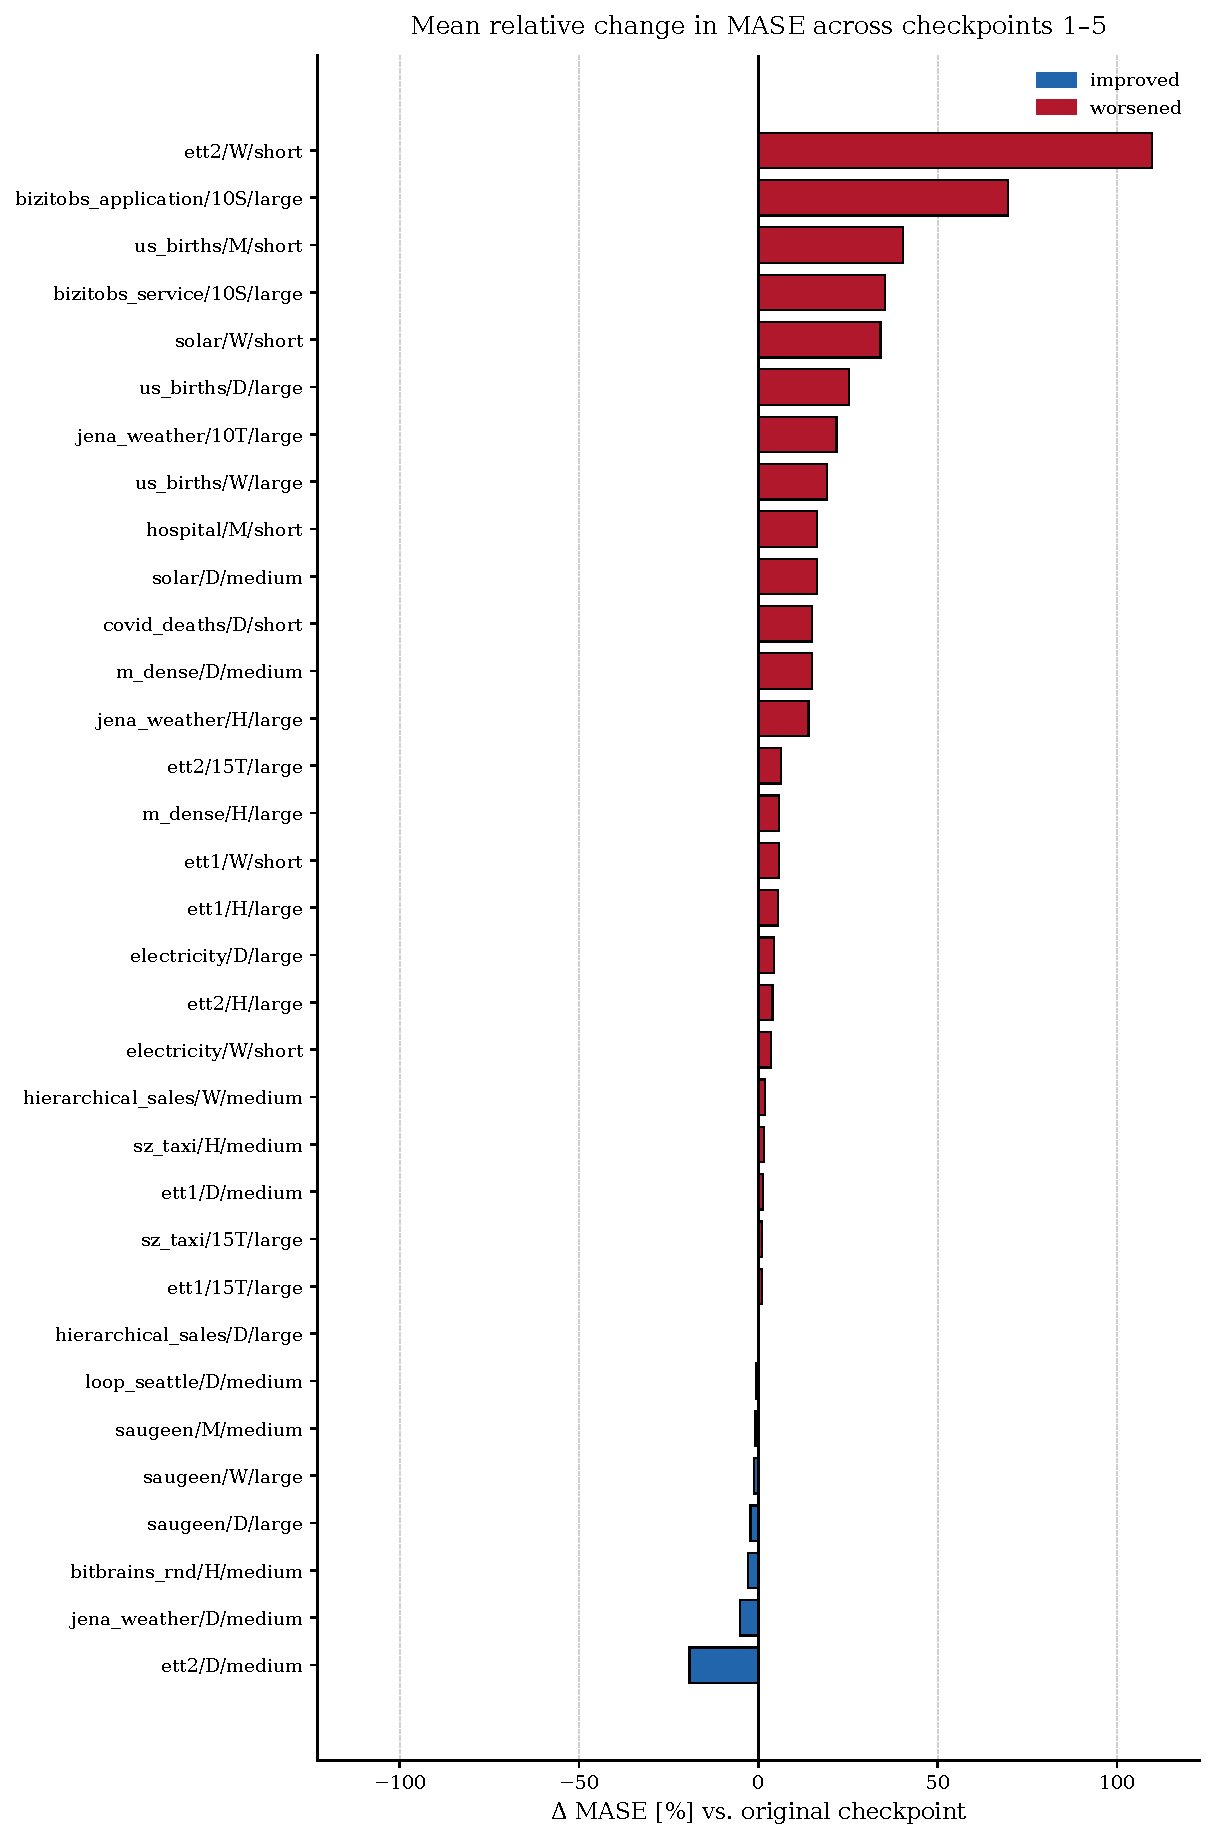
\includegraphics[width=\linewidth]{pictures/prior/mase_mean_delta_plot.pdf}
        \caption{Mean delta over all checkpoints}
        \label{fig:mase_mean_delta_plot}
    \end{subfigure}
    \hfill
    \begin{subfigure}[t]{0.3\textwidth}
        \centering
        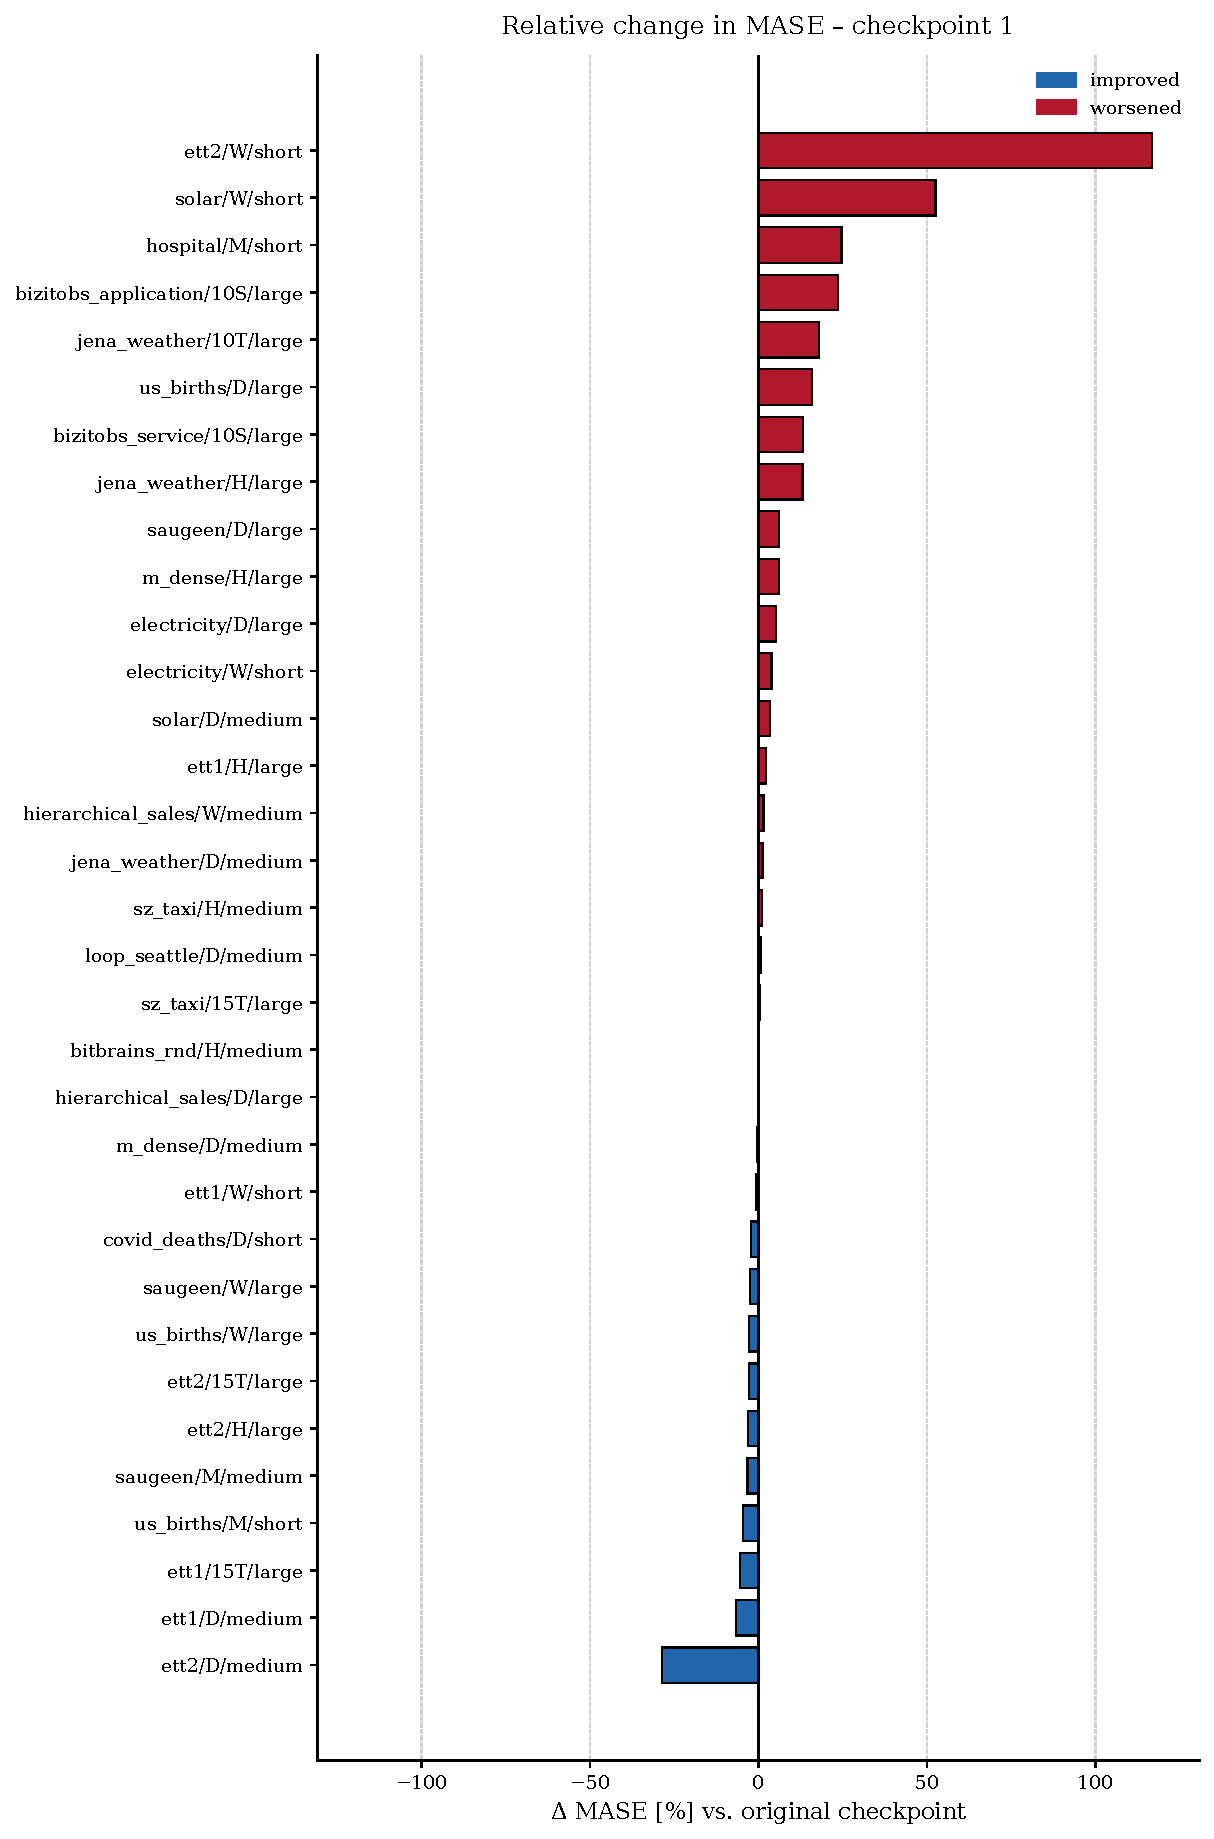
\includegraphics[width=\linewidth]{pictures/prior/mase_ckpt_1_delta_plot.pdf}
        \caption{Delta of checkpoint 1}
        \label{fig:mase_ckpt_1_delta_plot}
    \end{subfigure}
    \hfill
    \begin{subfigure}[t]{0.3\textwidth}
        \centering
        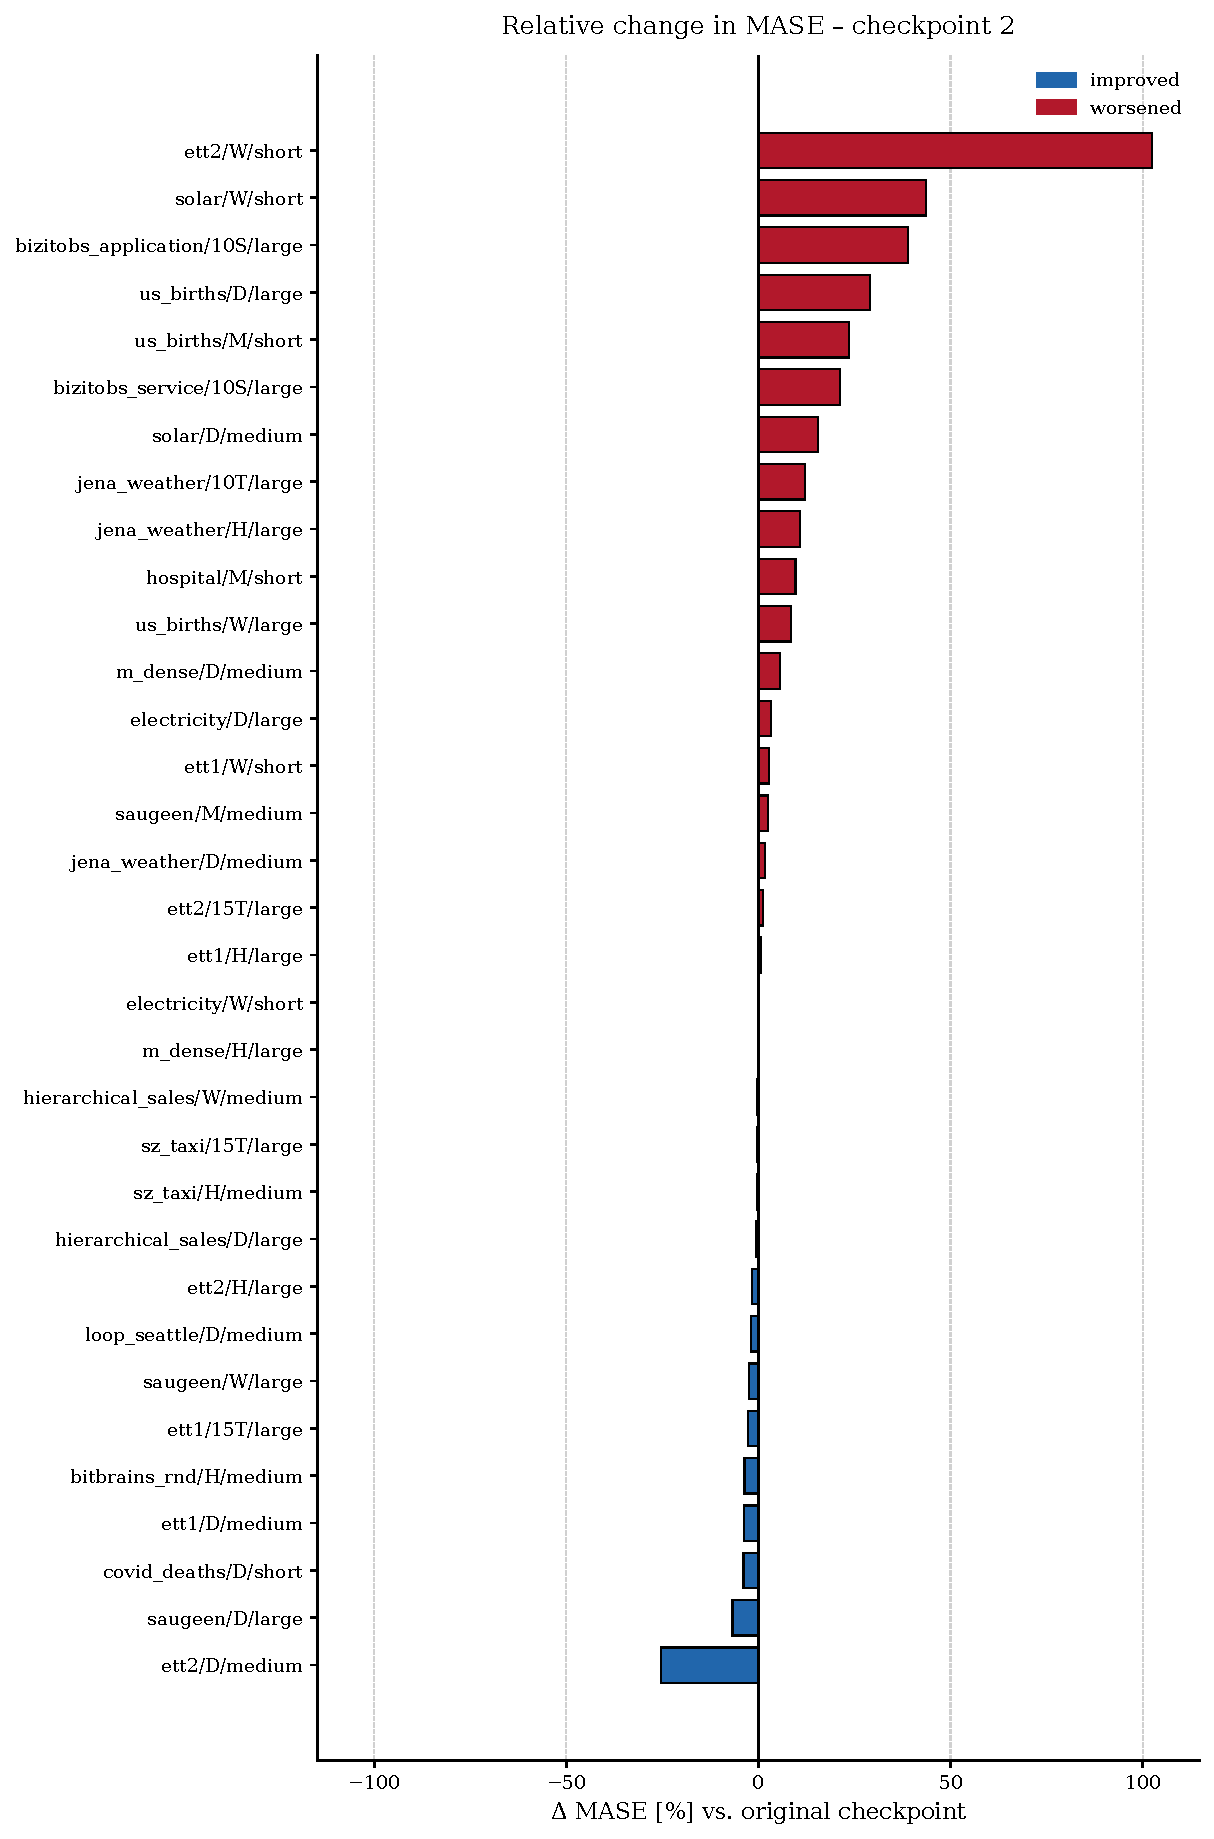
\includegraphics[width=\linewidth]{pictures/prior/mase_ckpt_2_delta_plot.pdf}
        \caption{Delta of checkpoint 2}
        \label{fig:mase_ckpt_2_delta_plot}
    \end{subfigure}

    \vspace{0.5cm}

    \begin{subfigure}[t]{0.3\textwidth}
        \centering
        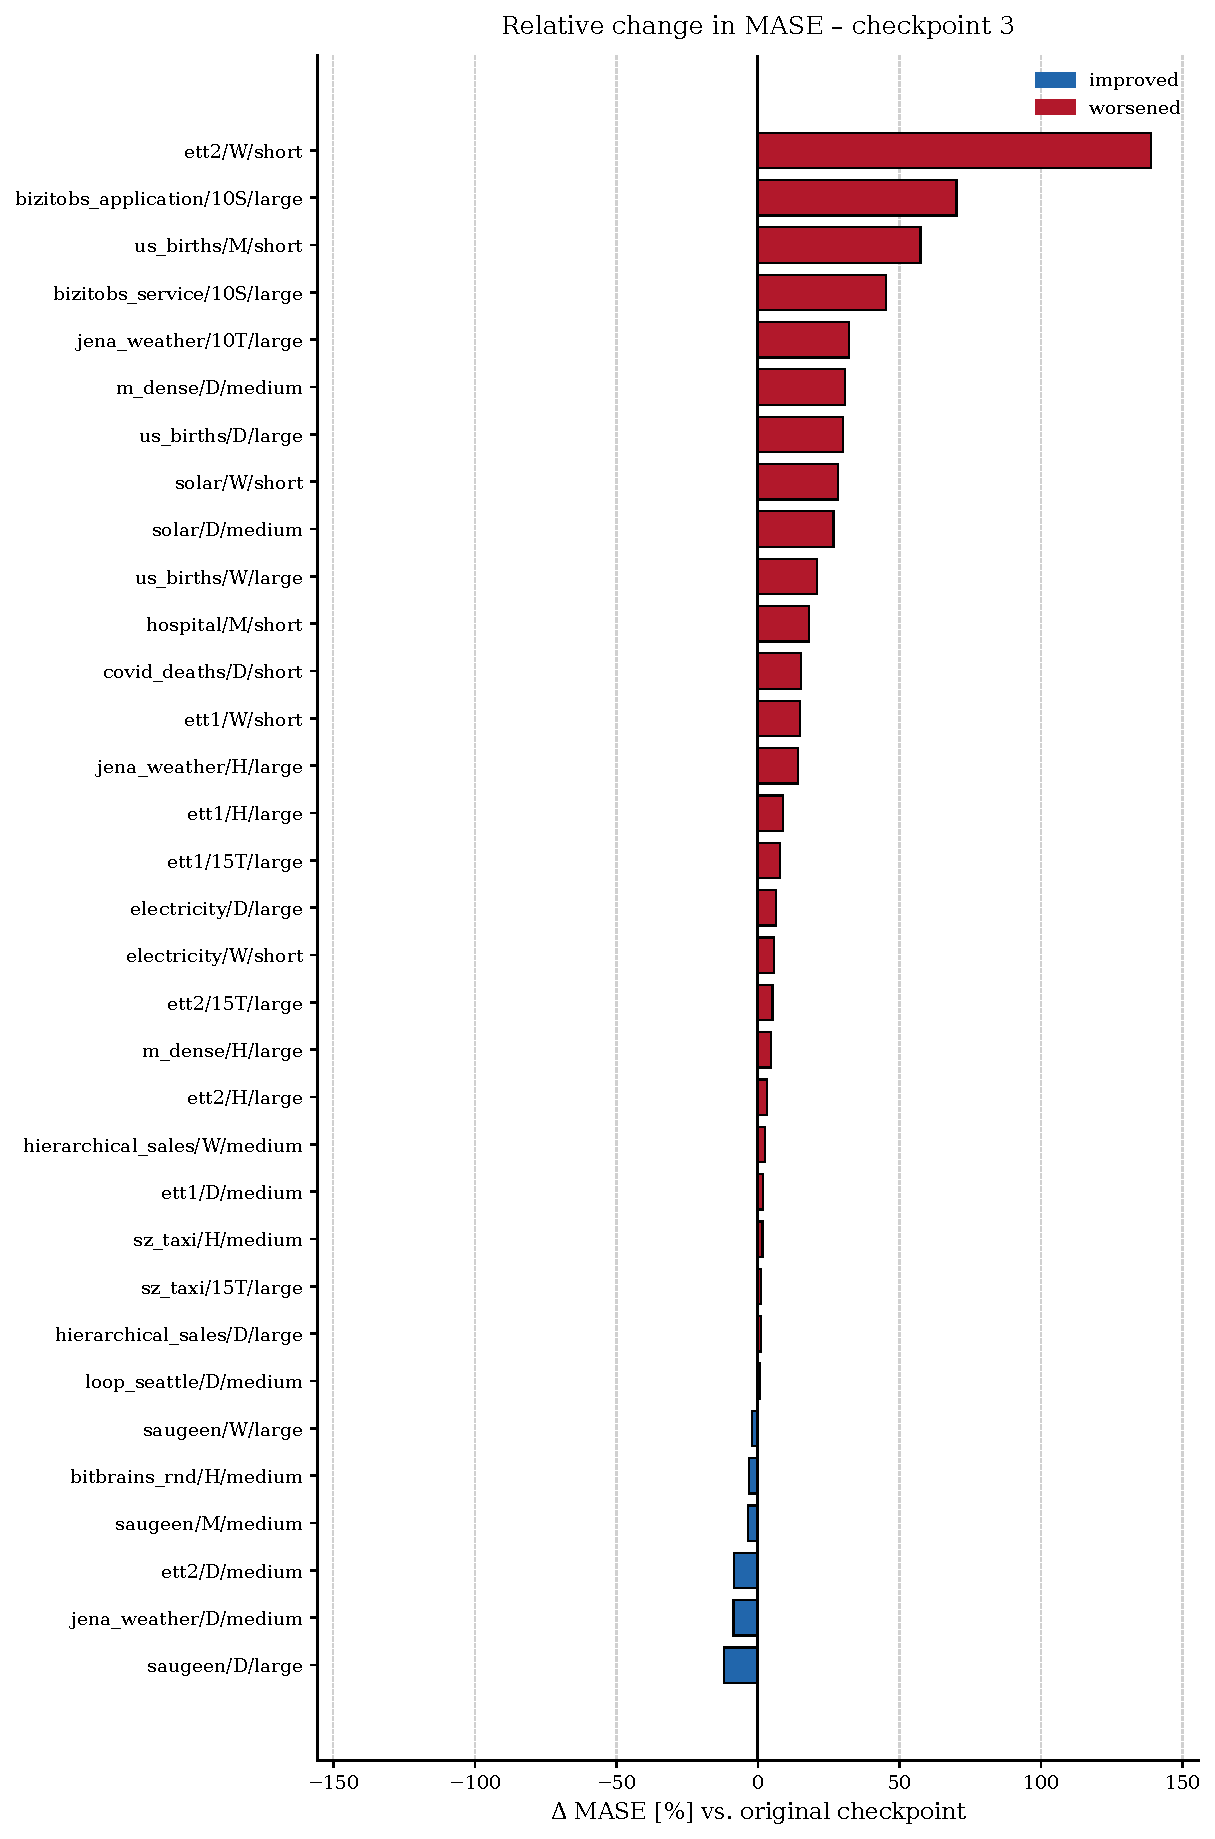
\includegraphics[width=\linewidth]{pictures/prior/mase_ckpt_3_delta_plot.pdf}
        \caption{Delta of checkpoint 3}
        \label{fig:mase_ckpt_3_delta_plot}
    \end{subfigure}
    \hfill
    \begin{subfigure}[t]{0.3\textwidth}
        \centering
        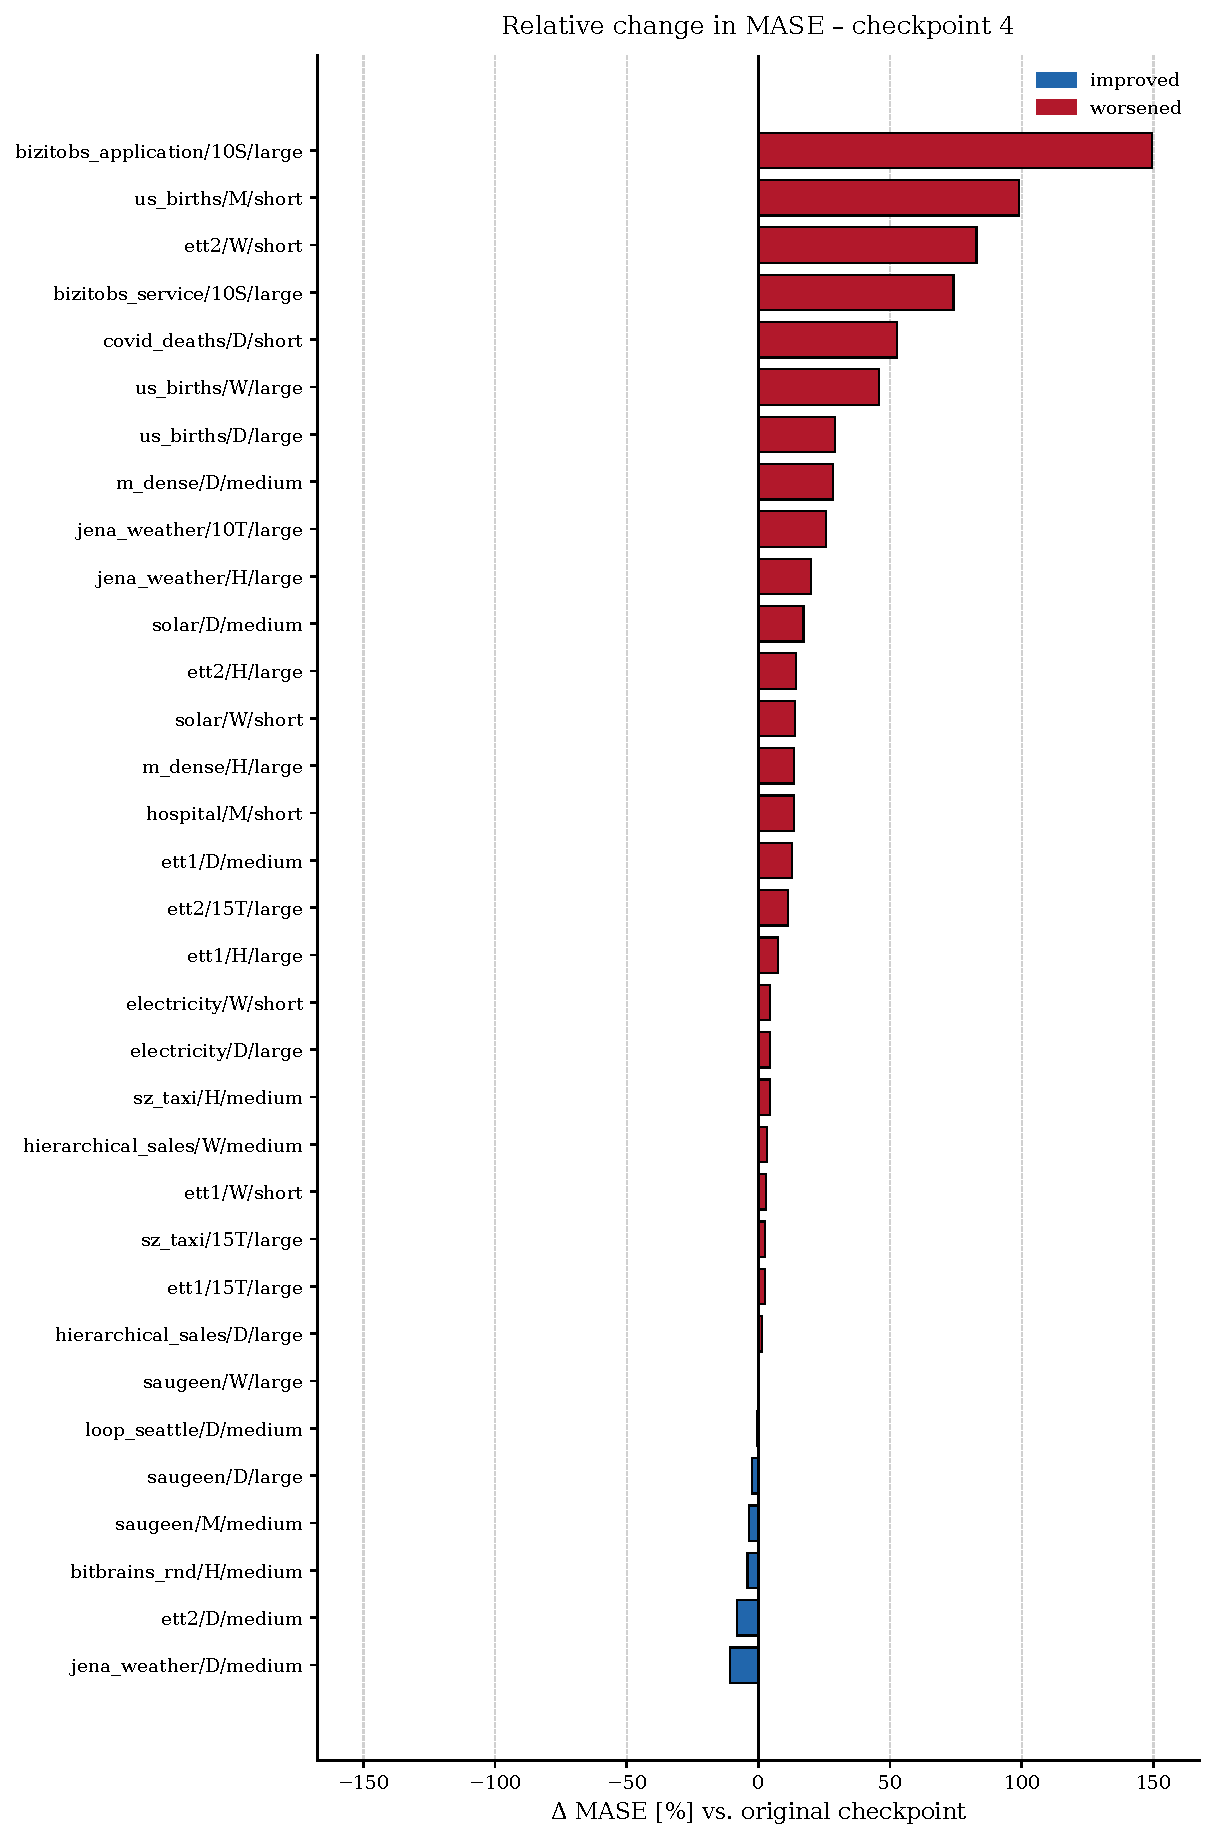
\includegraphics[width=\linewidth]{pictures/prior/mase_ckpt_4_delta_plot.pdf}
        \caption{Delta of checkpoint 4}
        \label{fig:mase_ckpt_4_delta_plot}
    \end{subfigure}
    \hfill
    \begin{subfigure}[t]{0.3\textwidth}
        \centering
        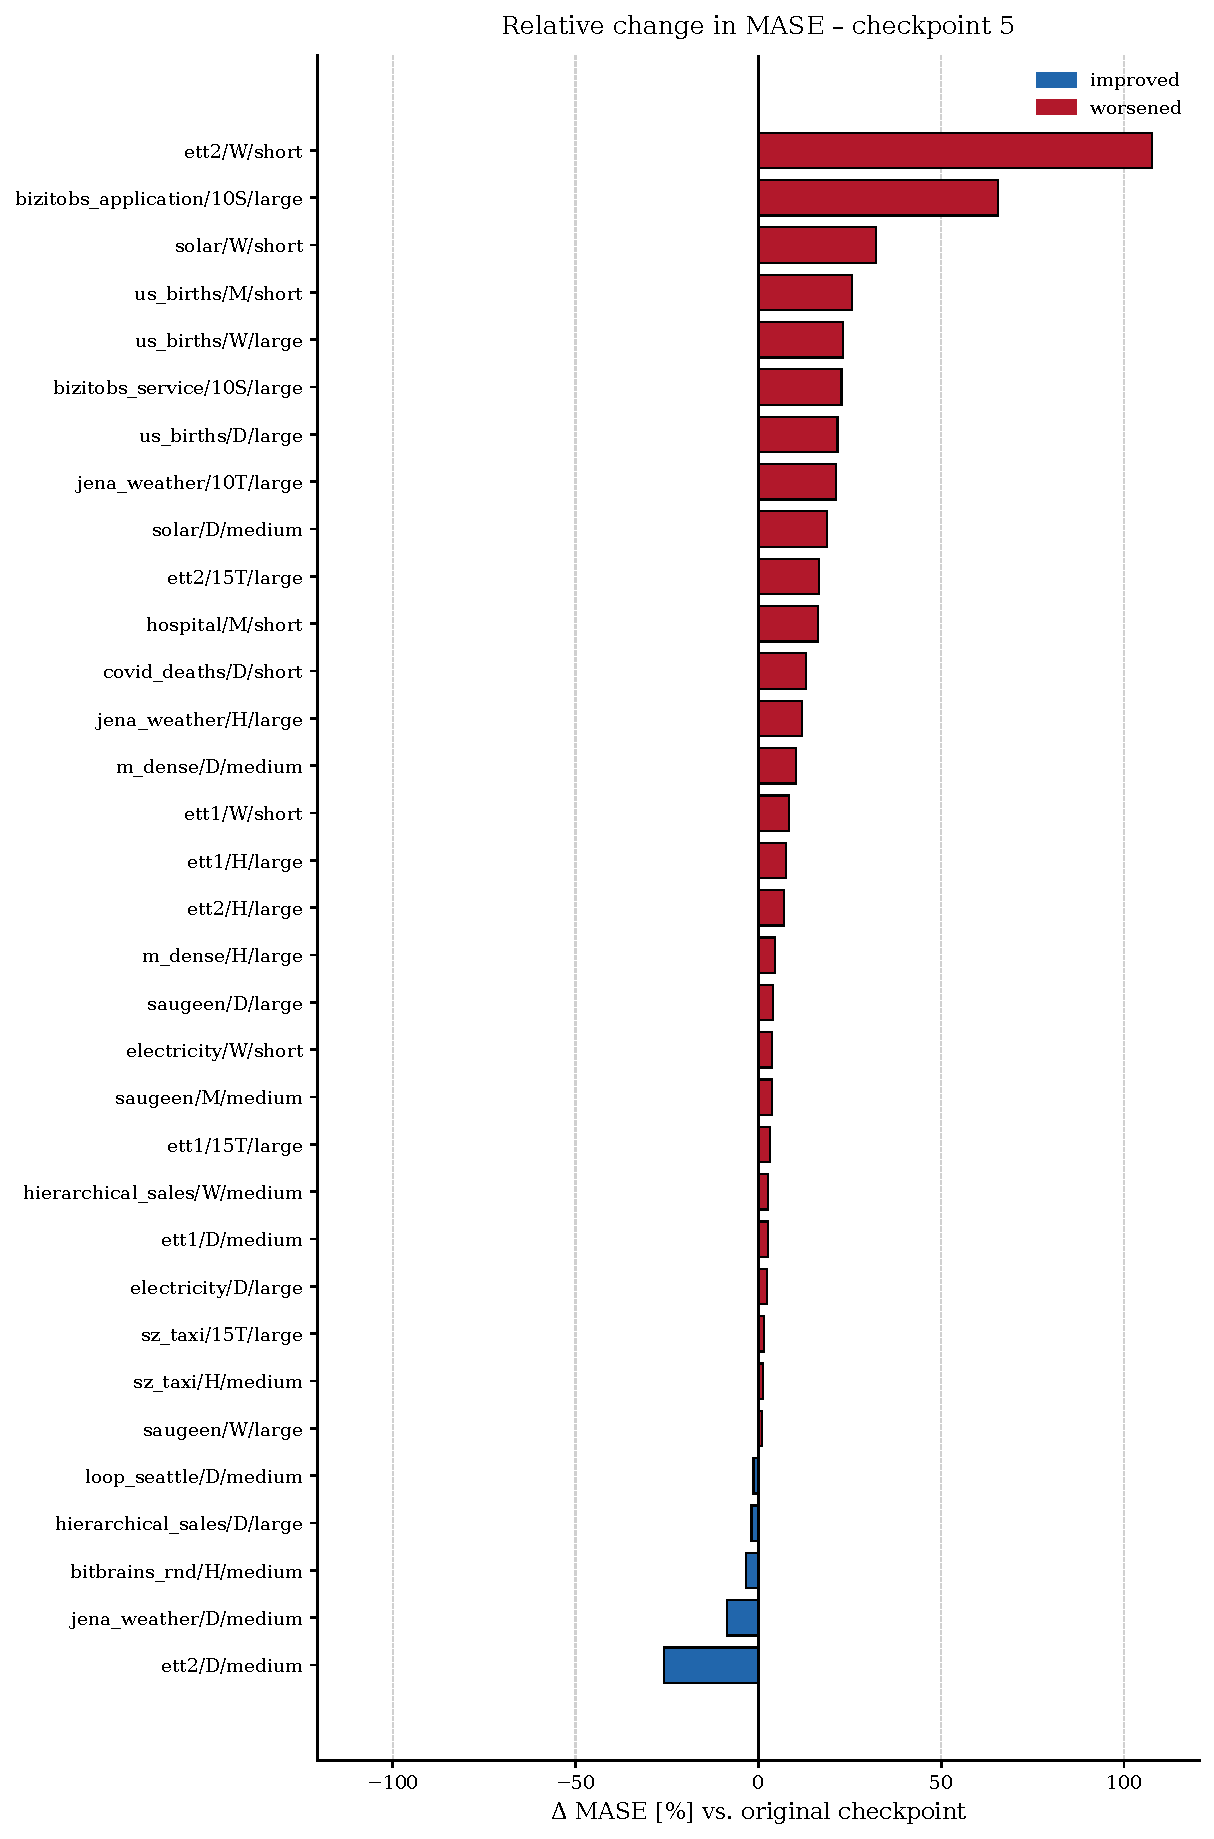
\includegraphics[width=\linewidth]{pictures/prior/mase_ckpt_5_delta_plot.pdf}
        \caption{Delta of checkpoint 5}
        \label{fig:mase_ckpt_5_delta_plot}
    \end{subfigure}

    \caption{Comparison of mean and checkpoint-wise delta plots. Lower is better. }
    \label{fig:combined_delta_plots}
\end{figure}
As shown in Figure~\ref{fig:mase_mean_delta_plot}, the mean performance across all five checkpoints improves on only three datasets, while it deteriorates on the remaining ones.
However, when analyzing individual checkpoints, differences become apparent. Checkpoints 1 and 2 both improve performance on 9 out of 18 datasets, whereas checkpoints 3, 4, and 5 show improvements on only a small number of datasets.
Furthermore, the improvements vary noticeably across datasets. While some datasets show noticeable gains, others exhibit negligible changes or even significant performance degradation.

The results also indicate that the effect of continued pretraining is highly dataset-dependent.
For example, datasets such as \textit{ett2/D} show consistent improvements across multiple checkpoints, whereas others such as \textit{ett2/W} and \textit{solar/W} do not benefit from continued pretraining at all.
Notably, datasets with shorter context lengths, such as \textit{solar/W} (context length 52), appear to be particularly challenging.

\iffalse
As one can see in plot~\ref{fig:mase_mean_delta_plot}, the mean performance over a selected set of datasets improved only on three datasets but worsened on all others.
This is a result of averaging the MASE scores over all 5 selected checkpoints.
Checkpoints 1 and 2 in the selection improved better as they both improved on 9 datasets.
But some of this performance is so minimal that one can say it stayed the same.
Another thing that is interesting to observe is that continued pretraining does not work on some datasets at all.
These are, for example, ett2/W and solar/W.
Both of which are datasets that have a short context length (103 and 52)
\fi
% Erster und zweiter Checkpoint performt auf mehreren Datensets gut aber hat auf manchen auch sehr starke Verluste

% Andere 3 Checkpoints sind viel schlechter zt -> nur auf 2 Datensets maximal

% Es gibt Datensets, auf denen der Prior generell gut ist, und manche, auf denen er überhaupt nicht gut ist.


\begin{table}[H]
\centering
\resizebox{0.8\textwidth}{!}{
\begin{tabular}{lcccccccccccccc}
\hline
Ckpt & Time & LR & Batch & L2-SP & WD & Time & Init & Best & Last & Steps & Best & ES & Time/ & Util \\
     & Limit &     &       &       &     & Spent & Val & Val & Val &       & Step &    & Step  &      \\
\hline
ckpt\_1 & 3600 & 0.0005 & 8 & 0.0001 & 0.0 & 3578.13 & 0.3624 & 0.2636 & 0.3315 & 115 & 79  & Time     & 31.11 & 35.33 \\
ckpt\_2 & 3600 & 0.0005 & 8 & 0.0    & 0.0 & 3585.33 & 0.3624 & 0.2762 & 0.2899 & 114 & 89  & Time     & 31.45 & 33.89 \\
ckpt\_3 & 3600 & 0.0005 & 2 & 0.0001 & 0.0 & 3603.73 & 0.3624 & 0.2812 & 0.2905 & 427 & 289 & Time     & 8.44  & 14.52 \\
ckpt\_4 & 3600 & 0.0005 & 2 & 0.0015 & 0.0 & 3336.01 & 0.3624 & 0.2861 & 0.5537 & 400 & 189 & AdaptES  & 8.34  & 14.19 \\
ckpt\_5 & 3600 & 0.0005 & 4 & 0.0    & 0.0 & 3669.10 & 0.3624 & 0.2912 & 0.2912 & 250 & 249 & Time     & 14.68 & 20.05 \\
\hline
\end{tabular}
}
\caption{Training results across checkpoints.}
\label{tab:training_results}
\end{table}
Table~\ref{tab:training_results} summarizes the hyperparameter configurations and training results of the top five checkpoints.
All selected checkpoints were trained with a learning rate of 0.0005. Configurations using smaller learning rates (e.g., 0.00005 and 0.000005) resulted in consistently worse validation performance and were therefore not included among the top checkpoints.
Regarding batch size, the top-performing checkpoints (ckpt\_1 and ckpt\_2) were trained with a batch size of 8, while other checkpoints used batch sizes of 2 or 4.
Additionally, a difference in the number of training steps can be observed. Checkpoints 1 and 2 performed significantly fewer steps (approximately 115) compared to checkpoints 3–5, which executed up to 427 steps.

Another notable observation is that four out of five checkpoints stopped training due to the time limit rather than early stopping based on validation performance.
Only checkpoint 4 terminated due to early stopping (AdaptiveES), indicating that most runs were constrained by the predefined training time.

\iffalse
By looking at table~\ref{tab:training_results}, one can see that all five checkpoints were trained with a learning rate of 0.0005.
The other checkpoints that yielded worse validation loss were mostly trained with learning rates smaller than this (0.00005, 0.000005), as shown in~\ref{TODO}.

Another interesting aspect is the step amount.
As mentioned above, the first two checkpoints performed significantly better on multiple datasets than the last three.
These two checkpoints also happen to have many fewer steps than the last three.
While ckpt\_1 and ckpt\_2 have a total of 115 and 114 steps, ckpt\_3, ckpt\_4, and ckpt\_5 have at least double the number of steps.
A cause for this could possibly be that the batch size of checkpoints 1 and 2 is both 8, thus needing more data to generate (that is why they also need double the time)
But they also perform significantly better.
Batch size 8 seems to be superior.
Another thing that comes to mind is that 4 of 5 checkpoints stopped training due to the time limit, not because the validation loss did not improve.
This is another important factor since ckpt\_1 and ckpt\_2 both needed much more time per step and could possibly improve even more
\fi
% hier so wie Single-Finetuning-Graphen und so zeigen weil ist ja nicht viel anders und wir haben auch viele Datensets

% Scatterplot mit x original und y prior MASE-Wert und diagonale
% prozentual Plot der Verbesserung zeigen Balkendiagramm

% Performance von 1. Checkpoint alleine auch zeigen
% vielleicht auch Performance von allen anderen Checkpoints auch zeigen



% Viele Trainingsläufe haben nicht aufgehört weil Patience auslief sondern weil Zeit vorbei war
% beste HP Konfig auf jeden Fall mit 0.0005 lr
\section{Discussion}
In our expose we defined the following question for this section:
"Can we continue pre-training TabPFN for time series with a prior that generates time series data (and does it improve performance)?"
This question can be answered positively, although the results indicate limitations, and the approach does not perform as well as initially expected.

A prior for time series should be able to generalize across different time series characteristics and yield better, more consistent results.
However, in our case with the prior we used from \citep{dooley2023forecastpfn}, this is not the case, as the effect we observed is very heterogeneous and, on average, only leads to better results on a small number of datasets.
A worsening of TabPFNs' performance is an effect we are looking at.
In the results section and what can be seen in <fig ref>, we can conclude that TabPFN only improved on 4 datasets but deteriorated on 20 other datasets.
These results alone are not sufficient to conclude that training with these prior results results in improved performance.

An especially interesting aspect was the behavior of the five checkpoints we selected based on their validation loss during training.
Checkpoints 1 and 2 perform significantly better than the other three checkpoints.
TabPFN improved performance on 12 and 11 datasets using these two checkpoints.
This suggests that these two checkpoints have different characteristics during training that allowed them to better adapt to the time series training data.

If we take a look at the hyperparameters that were used for the five checkpoints, we can observe that both of the top checkpoints used a batch size of 8, contrary to the other three, which used 2 and 4.
Empirically, this lets us assert that a batch size of 8 with a learning rate of 0.0005 is a good hyperparameter configuration for continued pretraining.

The training duration, measured by the number of steps/epochs we trained TabPFN on, also helps us conclude on another important factor for continued pretraining.
Both checkpoints 1 and 2 were trained for a total of 114/115 steps and reached their best performance at steps 79 and 89.
The other three checkpoints trained significantly longer, with up to 400 steps, while reaching their best state at step 189.
The consistently stronger performance of the early checkpoints suggests that moderate continued pretraining may be beneficial, while prolonged training may instead be harmful.
\newline
All checkpoints also ended due to the time limit of at most 40 minutes, instead of early stopping due to no improvements regarding the validation loss.
On the one hand, the reaching of this time limit comes from the data generation that is done dynamically while training.
On the other hand, this suggests that, since all runs were terminated due to the time limit rather than exhausted patience, the current results may not yet fully reflect the method’s potential.

For some datasets, it can be observed that the performance of all checkpoints consistently deteriorates, whereas for others it consistently improves.
This suggests that, while evaluation can also be different between checkpoints, it is also dataset-dependent.
Datasets that only experience a worsening mostly show difficult characteristics, such as noisy or intermittent time series, that even initially make it hard for TabPFN to forecast.

Finally, we can conclude that continued pretraining with a time-series-generating prior shows promising results, but it is not as general as one might think.
Our work here is limited only to the prior constructed by \citep{dooley2023forecastpfn}.
Future work should also focus on other time-series priors, as the general concept of further training a model with artificial time-series data yielded acceptable results.
% 1. High-level conclusion
% 2. Overall prior effect (heterogeneous)
% 3. Checkpoint behavior (early vs late)
% 4. Hyperparameter sensitivity
% 5. Training constraints (time limit)
% 6. Dataset dependency (datasets that don't perform well don't have the specific time series characteristic)

% prior effect nicht so wie gewünscht
% eher selektiv als globale Verbesserung
% heterogene statt homogene Effekte

% dataset dependent

% Checkpoints unterschiedlich -> frühe Checkpoints waren hier besser was darauf hindeuten kann dass mehr Training nicht gleich besser ist
% effizientes Training besser

% sehr hyperparameter empfindlich
% zu große Batch Sizes führen zu nichts und brauchen zu lange
% zu kleine Learning Rate zu konservativ

% Die konsistent besseren Ergebnisse der frühen Checkpoints deuten darauf hin, dass moderates Continued Pretraining nützlich sein kann, während längeres Training eher schadet.
% „Da alle Runs durch das Zeitlimit und nicht durch ausgeschöpfte Patience beendet wurden, ist es plausibel, dass die derzeitigen Ergebnisse das Potenzial der Methode noch nicht vollständig abbilden.“

% für manche Datensets stellt der Prior die Verteilung besser dar als für andere


% Conclusion bzw eher an den Anfang und Frage beantworten
% prior führt nicht zu einer klaren Verbesserung auf allen Datensets sondern hat eine Art Trade-off
% auf manchen Datensets wird es viel besser und auf manchen gar nicht
% hängt auch oft von der zugrunde liegenden Veteilung ab die ein Datenset hat und die des Prior

\chapter{Conclusion}
\label{chap:conclusion}
This thesis focused on evaluating three methods to potentially enhance TabPFN’s performance on time series data.
While \citet{hoo2025tables} already demonstrated promising results on time series forecasting, we aimed to further improve this performance.
We first tried to finetune TabPFN on one dataset from the GIFT-Eval benchmark of \citet{aksu2024giftevalbenchmarkgeneraltime} individually, and after that, evaluated the performance impact.
\newline
In our second approach, we split the datasets into three categories based on their number of observations per time series: Small, Medium, and Large.
Then, selecting a few to train TabPFN with and a few to evaluate the trained model on.
\newline
Our final method consists of a prior provided by \citet{dooley2023forecastpfn}\footnote{The code of the prior is available at \url{https://github.com/abacusai/forecastpfn}}.
We continued pretraining TabPFN with artificial time series data to presumably improve its performance on such data.
\newline
Based on these results, we will now finally compare these outcomes to determine which scenario and which methods are to be preferred.
\section{Key Findings}
\iffalse
In this section, we summarize the key findings of our experiments on finetuning and continued pretraining of TabPFN for time series forecasting.
While the results show that performance improvements are achievable, they also reveal important dependencies on data attributes, training strategies, and model configurations.

% Finetuning funktioniert – aber nur unter Bedingungen
As the results of finetuning on one dataset show, it does work.
But it is highly dependent on the dataset structure, as well as the context length and the amount of time series.
This
\fi
% Multi-Finetuning: Trade-off zwischen Generalisierung und Qualität
% Continued Pretraining: funktioniert, aber nicht general
% Validation Loss ist kein verlässlicher Indikator
% Dataset-Struktur ist entscheidend
% Data Scarcity: großer Vorteil von Multi & Prior

% Single finetunen wenn man genau weiß welche Daten da sind und man viele Daten hat
% Multi-Finetuning gut wenn man die grobe Struktur kennt und außerdem schon viele Trainingsdaten hat
% prior gut für wenn man keine Real-Life-Trainingsdaten hat und generalisieren will
In this section, we summarize the key findings of our experiments on finetuning and continued pretraining of TabPFN for time series forecasting.
While the results show that performance improvements are achievable, they also reveal important dependencies on data attributes, training strategies, and model configurations.

As the results of finetuning on a single dataset show, TabPFN can be successfully adapted to time series data. However, its effectiveness is highly dependent on the structure of the dataset, in particular, the number of time series, the available context length, and the overall amount of observations.
Datasets with many time series and sufficient context length consistently benefit from fine-tuning, whereas datasets with only a few series or limited structure often show little to no improvement, or even performance degradation, indicating potential overfitting on these datasets.

Across all experiments, the validation loss proved to be an unreliable indicator for evaluation performance.
In many cases, checkpoints with lower validation loss did not correspond to better results in terms of MASE, indicating both a mismatch between training and evaluation metrics and a tendency to overfit the validation data.
In this context, overfitting to the validation data means that the model adapts too closely to the specific validation samples, reducing its ability to generalize to unseen test data.

The structure of the dataset itself holds a crucial role.
Time series with clear patterns, such as periodicity or consistent trends, are easier for TabPFN to learn, whereas noisy or intermittent datasets remain challenging for all methods.
This highlights that not all datasets are equally suitable for finetuning and that the underlying data distribution strongly influences the outcome.

When extending finetuning to several datasets, a trade-off between generalization and performance becomes clear.
Finetuning on small-context datasets leads to a deterioration in performance, likely due to insufficient information per sample.
In contrast, datasets with medium context lengths provide the best balance, letting the model generalize while still capturing meaningful structures.
Larger context datasets also yield improvements, but not as consistently as the medium category.

Continued pretraining with artificially generated time series shows that improvements are possible, but not equally across datasets.
The results are highly heterogeneous and strongly depend on the chosen prior and training configuration.
In particular, shorter training durations and specific hyperparameter choices tend to perform better, suggesting that prolonged training can harm performance rather than improve it.

Finally, an important observation is the benefit of multi-dataset finetuning and prior-based training under scenarios with limited data.
While single-dataset finetuning performs best when sufficient and well-structured data is available, multi-dataset approaches and prior-based methods achieve better performance in data-scarce settings by enabling greater generalization.

Our final question in the expose was "Which one of the following models performs best on various high-scale benchmarks: TabPFN-TS, finetuned TabPFN-TS, or continued pre-trained TabPFN-TS?"
Overall, the experiments and our complete evaluation in Table~\ref{tab:main_results_all_methods} in the appendix show that no single training strategy dominates in all scenarios.
Instead, the choice between single finetuning, multi-dataset finetuning, and continued pretraining should be based on the availability, structure, and quality of the underlying data.



% Hier noch Balkendiagramm für alle Datasets oder ein paar mit 3 Balken pro Datenset 1 für jede Methode
% einmal mit Average von den 5 immer
% und einmal mit Checkpoint vom besten Prior Training und bestem Checkpoint bei Multi

% Tabellen mit Zeilen Datenset und Spalten MASE von Single Multi und Prior


% prior mit Trade-off ganz gut
% Single finetuning auch für selektive am besten aber halt auch nur für das Datenset

% Multi auch nicht schlecht
% prior schneller weil keine hp Search gemacht werden muss

% tabpfn tut sich schwer auf Daten die keine klare Periodicitäten haben

% Vorteil den halt continued Pretraining und Multi-Finetuning mit sich mitbringt ist dass auf kleinen Datensets auch gut performed werden kann

\section{Limitations}
This work is subject to several limitations that should be considered when interpreting the results.

A major limitation is related to the datasets used in this thesis.
The selected datasets do not cover all possible types of time series and therefore only provide a limited perspective.
%As a result, the findings mainly show whether finetuning works for these selected datasets, but do not fully generalize to all possible real-life scenarios.
In particular, datasets with high irregularity or non-stationary behavior are underrepresented, meaning that the observed benefits of finetuning may not transfer to domains such as financial time series or event-driven data.
In addition, some datasets may inherently be less suitable for finetuning, for example, due to noisy, irregular, or difficult-to-model distributions.
This makes it harder for TabPFN to learn relevant patterns and limits the achievable improvements.

Another limitation concerns reproducibility.
The original evaluation scores from prior work could not be fully reproduced, which makes a direct comparison to reported results difficult.
This may be due to missing implementation details, differences in preprocessing, or stochastic training effects, which were not fully controllable in our setup.
Instead, comparisons in this thesis are based on internally consistent baseline results, which still allow for relative evaluation but limit comparability to external benchmarks.

A key limitation of the experimental setup is the mismatch between the validation objective (MSE) and the evaluation metric (MASE).
As observed in the results, this leads to weak alignment between checkpoint selection and final benchmark performance.

Furthermore, the experiments were conducted under computing limitations.
Finetuning runs were limited to a maximum runtime of 2400 seconds, and continued pretraining was also restricted by a fixed time limit.
This likely prevented some runs from fully converging and may have impacted the final performance.

Finally, it should be noted that a newer version of TabPFN (TabPFN 2.5) was released by \citet{grinsztajn2025tabpfn} after we had already decided to use the \textit{tabpfn-v2-regressor-2noar4o2} checkpoint, as it was also done in \citet{hoo2025tables}.
The experiments presented here are based on this checkpoint, and it is possible that some of the observed limitations or behaviors have already been improved in the newer model.

In general, these limitations show that while the results present useful insights, they should be interpreted with caution and seen as an initial study rather than a definitive evaluation.



% Dataset-Limitierungen
% Datasets don't fit for every situation, so it's hard to generalize since finetuning could work better with a better dataset
% Manche Datensets sind vielleicht einfach nicht gut zum Finetunen bzw. man kann tabpfn darauf nicht gut finetunen, weil die Verteilung einfach nicht gut zu approximieren ist
% Datasets only show a limited perspective und zeigen keine Generalisierung sondern nur ob finetuning mit diesen funktioniert oder nicht

% Reproduzierbarkeit
% Originalevaluationwerte konnten nicht alle reproduziert werden
% Deswegen ist eine direkte Vergleichbarkeit mit den Werten online nicht möglich nur mit den Werten die wir hier als Basewerte haben

% tabpfn 2.5 wurde währenddessen released was die was alle Ergebnisse die wir hier haben nochmal verbessert

% computing constraints von 2400 sek
% und time limit von continued pretraining

% Computing Constraints

% Generalisierbarkeit
\iffalse
- Die Forecast Windows sind manchmal nicht ganz passend für die Periodicitäten. Siehe us\_births
-
-
- Wir konnten nicht die original mase scores alle reproduzen
- time limit of continued pretraining
- prior vor allen Dingen gut bei data shortage
- ansonsten sprechen für Spezifizierung und viel Daten viel für Single und sonst für Multi

- Short ist gar nicht so gut
\fi

\section{Outlook}
While this thesis provides insight into different methods for fine-tuning TabPFN on time series data, further exploration of this topic would benefit from more extensive evaluation methods.

Improving the evaluation procedure could yield better results.
Even though the validation and evaluation setups are already quite similar, the results showed that validation accuracy does not always reflect the actual evaluation performance well.
Adjusting the validation metric or making the validation process more robust could help select better configurations.

Another important aspect is the dataset selection for multi-dataset finetuning.
In this work, we only tested a limited number of dataset combinations.
In particular, systematically varying the proportion of small- and large-context datasets, as well as other characteristics such as noise levels, could help identify whether negative transfer occurs when mixing heterogeneous dataset types.

A systematic hyperparameter search was not conducted and may reveal more robust configurations.
Conducting such a search could help identify configurations that perform reliably across methods and reduce the need for extensive trial runs.

Combining the different approaches could also be interesting.
For example, continued pretraining with a prior could be combined with multi-dataset finetuning to benefit from both generalization and adaptation to real data.

An aspect not investigated in this work is the impact of newer model versions.
During the work on this thesis, a new version of TabPFN (TabPFN 2.5) was released by \citet{grinsztajn2025tabpfn}.
Evaluating the methods with this updated model could lead to different and perhaps improved results.

Another important aspect is the sensitivity of prior-based continued pretraining to hyperparameter choices, as even small changes in configuration can lead to significantly different outcomes, making it difficult to identify robust settings.
Furthermore, the prior used for continued pretraining could be improved, as it may not fully capture the diversity and structural properties of real-world time series.
More expressive synthetic data generation methods, such as time series data generation via generative models explored by \citet{lawrence2021dgp}, could help enrich the prior and improve TabPFN-TS performance.
At the same time, scaling to large real-world datasets remains an important direction, as demonstrated by \textit{TimeBench} introduced in \citet{liu2025sundial}, which comprises over a trillion observations.
Combining improved synthetic priors with large-scale real-world data, therefore, represents a promising direction for continued pretraining.
%Finally, the prior used for continued pretraining could be improved.
%The current prior does not capture all characteristics of real-world time series, which likely limits its effectiveness.
%Other time series generating algorithms like https://arxiv.org/pdf/2104.08043 could help improve TabPFN-TS performance by continuing pretraining with artifial data.
%While artificial time series data is one way of pretraining large models, big datasets are the other side.
%https://arxiv.org/pdf/2502.00816v2 introduced TimeBench: a dataset collection that comprises over a trillion observation points in total from various sources.

Overall, further work is needed to better understand when and how these methods work best and how they can be combined effectively.



% Validation Metric bzw Evaluation Metric anpassen -> geht jetzt schlecht weil viel Zeit verloren
% Obwohl Validation und Evaluation schon durch die Aufteilung von Gift Eval sehr close sind muss die irgendwie besser laufen

% Dataset-Selektion für Multi anpassen
% Das hat uns jetzt nur einen Einblick gegeben
% durch mehrere verschiedene Läufe könnte man den Einfluss von einzelnen Datensets in der Auswahl auf die Performance herausfinden

% Hyperparameter wurden noch gar nicht angeschaut
% Hier könnte man eine geeignete Hyperparameter-Kombination raussuchen die für eine Fine-Tuning-Methode am besten klappt um so Runs zu sparen

% Kombination von Methoden
% Prior + Multi

%Wie verhält sich das neue TabPFN-Modell (TabPFN 2.5) gegenüber finetuning mit den Methoden?
% tabpfn 2.5 ist ja erst rausgekommen als die Thesis schon geschrieben wurde

% einen besseren Prior entwickeln



% Dataset-Selektion anschauen
% Mehr runs generell für alles mache insbesondere beim Multi um eine bessere Datenbasis zu haben

% Hyperparameter besser anschauen

% Kombination der Methoden
% Einfluss neuer Modelle
% Bessere Priors entwickeln

\chapter{Appendix}
\begin{figure}[h]
    \centering
    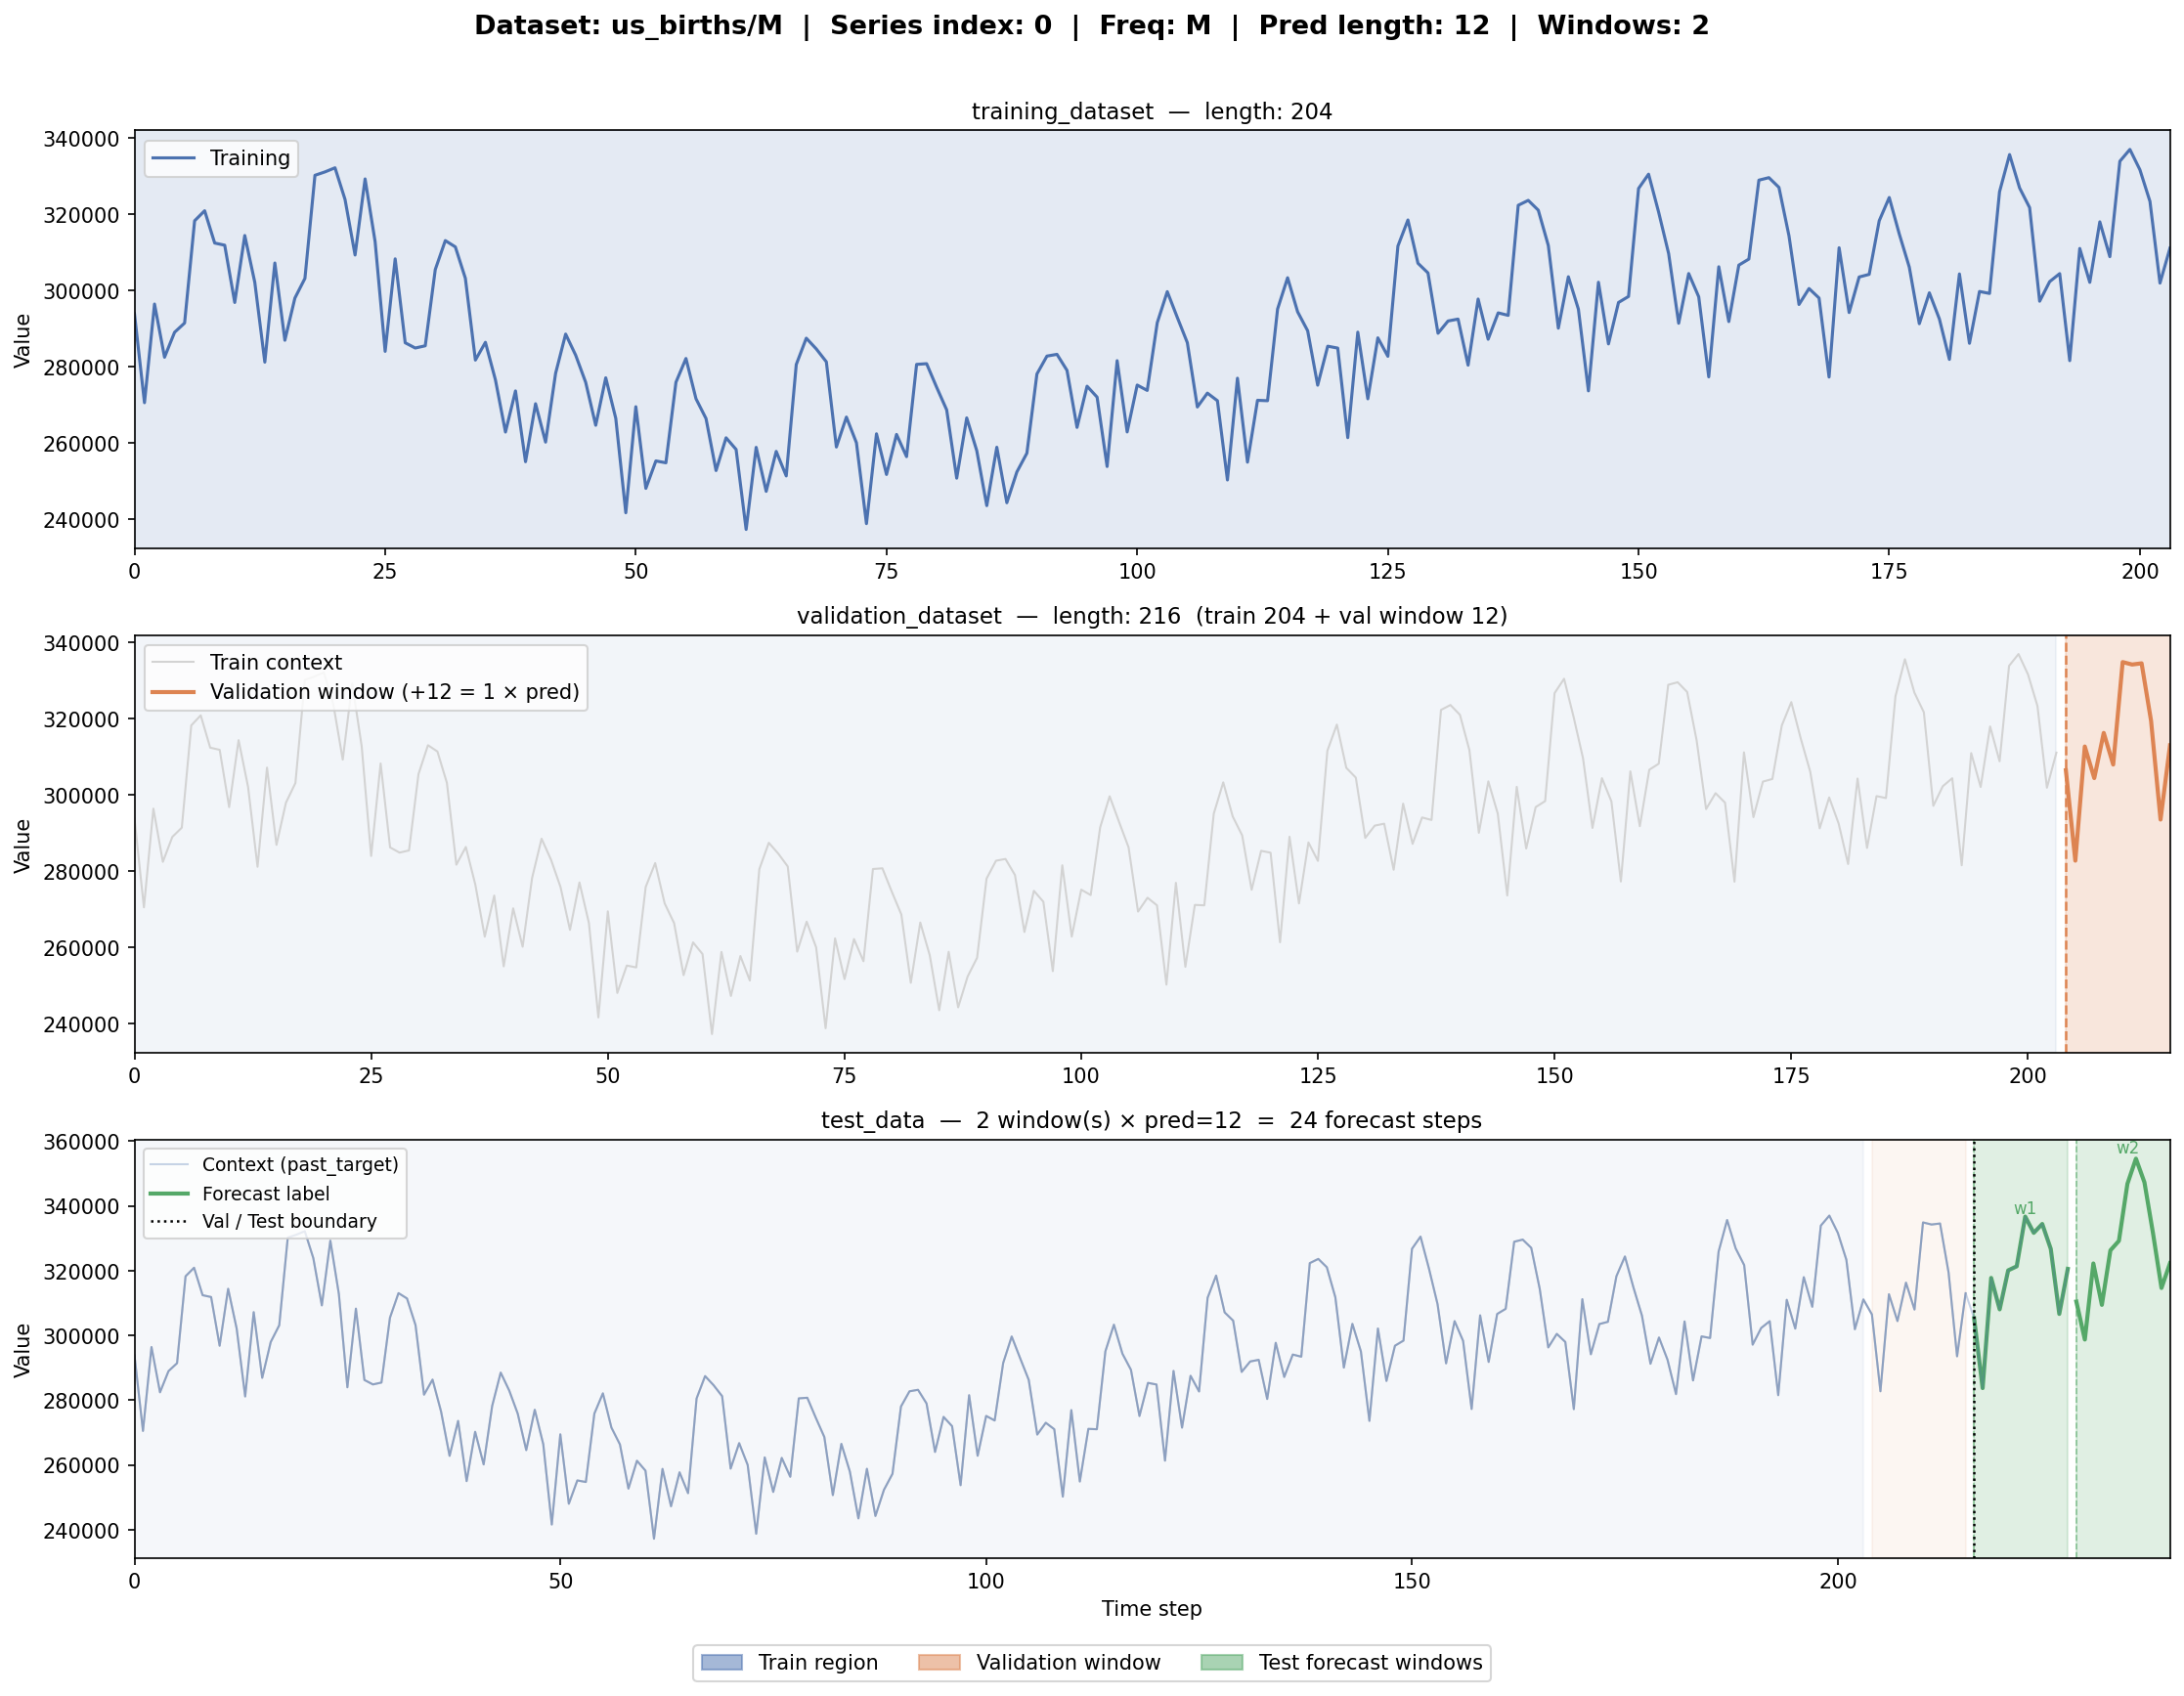
\includegraphics[width=0.8\textwidth]{pictures/splits_us_births_M_idx0.png}
    \caption{The three splits GIFT Eval provides to train and validate on a dataset while shadowing the test data for later benchmark evaluation.}
    \label{fig:gift_eval_split_us_births_m}
\end{figure}
- Tabelle mit allen Forecast Horizons und predictions lengths

\begin{table}[ht]
\centering
\resizebox{\textwidth}{!}{
\begin{tabular}{lrrrrrrrrrrr}
\toprule
Dataset & Context & Series & C1 & C2 & C3 & C4 & C5 & Mean $\Delta$ (\%) & Min & Max & Improved \\
\midrule
LOOP\_SEATTLE/D & 365 & 323 & -2.34 & -2.35 & -2.39 & -0.02 & -2.22 & -1.87 & -2.39 & -0.02 & True \\
M\_DENSE/D & 730 & 30 & 12.91 & 20.64 & 15.81 & 32.22 & 16.82 & 19.68 & 12.91 & 32.22 & False \\
M\_DENSE/H & 17520 & 30 & -1.80 & 1.56 & -2.07 & -3.05 & -6.37 & -2.35 & -6.37 & 1.56 & True \\
SZ\_TAXI/15T & 2976 & 156 & -1.81 & -1.83 & -1.78 & -1.85 & -1.75 & -1.80 & -1.85 & -1.75 & True \\
SZ\_TAXI/H & 744 & 156 & -2.20 & -2.26 & -2.26 & -1.68 & -1.26 & -1.93 & -2.26 & -1.26 & True \\
bitbrains\_rnd/H & 720 & 500 & -1.26 & -2.00 & -0.10 & -2.64 & -4.84 & -2.17 & -4.84 & -0.10 & True \\
bizitobs\_application & 8834 & 1 & 30.56 & 41.21 & 25.14 & 23.93 & 38.38 & 31.84 & 23.93 & 41.21 & False \\
bizitobs\_service & 8835 & 21 & 11.35 & -0.95 & 2.42 & 14.22 & 0.39 & 5.48 & -0.95 & 14.22 & False \\
covid\_deaths & 212 & 266 & -12.04 & -11.24 & -9.59 & -5.16 & 8.93 & -5.82 & -12.04 & 8.93 & True \\
electricity/D & 1461 & 370 & -1.73 & 4.16 & -0.78 & -3.01 & -3.19 & -0.91 & -3.19 & 4.16 & True \\
electricity/W & 208 & 370 & 0.67 & 6.46 & 24.55 & 12.74 & -0.32 & 8.82 & -0.32 & 24.55 & False \\
ett1/15T & 69680 & 1 & 9.59 & 0.59 & 0.30 & 0.24 & 0.33 & 2.21 & 0.24 & 9.59 & False \\
ett1/D & 725 & 1 & 0.00 & 0.00 & 0.00 & 0.00 & 0.00 & 0.00 & 0.00 & 0.00 & False \\
ett1/H & 17420 & 1 & -3.19 & -2.37 & -4.32 & -2.68 & 2.21 & -2.07 & -4.32 & 2.21 & True \\
ett1/W & 103 & 1 & 1.83 & -5.12 & 1.39 & -9.28 & 5.12 & -1.21 & -9.28 & 5.12 & True \\
ett2/15T & 69680 & 1 & -6.24 & -2.65 & -4.48 & -0.10 & 6.09 & -1.48 & -6.24 & 6.09 & True \\
ett2/D & 725 & 1 & -5.99 & -21.12 & -13.92 & -34.08 & -12.36 & -17.49 & -34.08 & -5.99 & True \\
ett2/H & 17420 & 1 & -6.68 & -2.50 & -9.41 & -9.10 & -6.23 & -6.78 & -9.41 & -2.50 & True \\
ett2/W & 103 & 1 & 46.42 & 134.09 & 22.27 & 74.30 & 35.36 & 62.49 & 22.27 & 134.09 & False \\
hierarchical\_sales/D & 1825 & 118 & -0.60 & -0.60 & -0.60 & -2.39 & -2.24 & -1.29 & -2.39 & -0.60 & True \\
hierarchical\_sales/W & 260 & 118 & 1.07 & 4.49 & 4.44 & 4.39 & 1.68 & 3.22 & 1.07 & 4.49 & False \\
hospital & 84 & 767 & 2.71 & -0.48 & 1.98 & 0.89 & 0.66 & 1.15 & -0.48 & 2.71 & False \\
jena\_weather/10T & 52704 & 1 & 0.00 & 0.00 & 0.00 & 0.00 & 0.00 & 0.00 & 0.00 & 0.00 & False \\
jena\_weather/D & 366 & 1 & 21.54 & 4.78 & 4.63 & 3.76 & -0.17 & 6.91 & -0.17 & 21.54 & False \\
jena\_weather/H & 8784 & 1 & 5.22 & 3.20 & 1.30 & -0.54 & -1.45 & 1.54 & -1.45 & 5.22 & False \\
saugeenday/D & 23741 & 1 & -3.81 & -3.79 & -3.35 & -1.03 & -2.87 & -2.97 & -3.81 & -1.03 & True \\
saugeenday/M & 780 & 1 & 4.60 & 8.45 & 6.76 & 11.79 & 7.85 & 7.89 & 4.60 & 11.79 & False \\
saugeenday/W & 3391 & 1 & 7.98 & -2.58 & -1.07 & 11.83 & 9.89 & 5.21 & -2.58 & 11.83 & False \\
solar/D & 365 & 137 & 10.13 & 9.08 & 25.76 & 13.26 & 9.75 & 13.60 & 9.08 & 25.76 & False \\
solar/W & 52 & 137 & 99.83 & 108.15 & 109.70 & 157.05 & 178.98 & 130.74 & 99.83 & 178.98 & False \\
us\_births/D & 7305 & 1 & 54.45 & 17.03 & 17.05 & 17.03 & 10.24 & 23.16 & 10.24 & 54.45 & False \\
us\_births/M & 240 & 1 & 8.58 & 6.39 & 6.58 & 7.08 & 6.44 & 7.02 & 6.39 & 8.58 & False \\
us\_births/W & 1043 & 1 & 14.04 & -0.90 & 17.79 & 2.29 & -4.66 & 5.71 & -4.66 & 17.79 & False \\
\bottomrule
\end{tabular}
}
\caption{Vollständige Ergebnisse des Fine-Tunings über alle Datensätze und Checkpoints. Negative Werte entsprechen einer Verbesserung der Modellperformance.}
\label{tab:eval_score_single_finetune}
\end{table}



\begin{table}[htbp]
    \centering
    \caption{Mean Delta (\%) per Dataset}
    \label{tab:main_results}
    \begin{tabular}{lrrrrr}
        \toprule
        Dataset & Single & Multi Short & Multi Medium & Multi Big & Prior \\
        \midrule
        bitbrains\_rnd/H & -2.17 & -- & -1.70 & -- & \textbf{-2.89} \\
        bizitobs\_application & \textbf{31.84} & -- & -- & -- & 69.52 \\
        bizitobs\_service & \textbf{5.48} & -- & -- & -- & 35.28 \\
        covid\_deaths & \textbf{-5.82} & 26.75 & 15.58 & 48.80 & 14.92 \\
        electricity/D & \textbf{-0.91} & -- & -- & -0.68 & 4.33 \\
        electricity/W & 8.82 & 4.16 & -- & -- & \textbf{3.60} \\
        ett1/15T & 2.21 & -- & -- & \textbf{-5.80} & 1.03 \\
        ett1/D & \textbf{0.00} & -- & 2.21 & -- & 1.34 \\
        ett1/H & -2.07 & -- & -- & \textbf{-2.58} & 5.37 \\
        ett1/W & -1.21 & \textbf{-9.47} & -- & -- & 5.64 \\
        ett2/15T & \textbf{-1.48} & -- & -- & -0.30 & 6.27 \\
        ett2/D & -17.49 & -- & \textbf{-31.26} & -- & -19.23 \\
        ett2/H & \textbf{-6.78} & -- & -- & -0.90 & 3.89 \\
        ett2/W & \textbf{62.49} & 73.16 & -- & -- & 109.70 \\
        hierarchical\_sales/D & \textbf{-1.29} & -- & -- & -1.01 & -0.00 \\
        hierarchical\_sales/W & 3.22 & -- & \textbf{-0.30} & -- & 1.93 \\
        hospital/M & \textbf{1.15} & 2.68 & -- & -- & 16.43 \\
        jena\_weather/10T & \textbf{0.00} & -- & -- & -- & 21.76 \\
        jena\_weather/D & 6.91 & -- & 0.71 & -- & \textbf{-5.06} \\
        jena\_weather/H & \textbf{1.54} & -- & -- & -- & 13.99 \\
        loop\_seattle/D & -1.87 & 4.28 & -1.54 & \textbf{-2.27} & -0.53 \\
        m\_dense/D & 19.68 & -- & \textbf{2.22} & -- & 14.91 \\
        m\_dense/H & \textbf{-2.35} & 15.98 & -- & 0.28 & 5.71 \\
        saugeenday/D & \textbf{-2.97} & -- & -- & -1.00 & -2.23 \\
        saugeenday/M & \textbf{7.89} & -- & -0.45 & -- & \textbf{-0.81} \\
        saugeenday/W & \textbf{5.21} & -- & -- & -- & \textbf{-1.23} \\
        solar/D & 13.60 & -- & \textbf{0.07} & -- & 16.30 \\
        solar/W & 130.74 & \textbf{9.98} & -- & -- & 34.04 \\
        sz\_taxi/15T & \textbf{-1.80} & -- & -0.22 & 0.05 & 1.08 \\
        sz\_taxi/H & \textbf{-1.93} & -- & -1.04 & -- & 1.59 \\
        us\_births/D & \textbf{23.16} & -- & -- & 23.53 & 25.17 \\
        us\_births/M & 7.02 & -- & \textbf{-0.44} & -- & 40.20 \\
        us\_births/W & 5.71 & -- & \textbf{1.49} & -- & 19.10 \\
        \bottomrule
    \end{tabular}
\end{table}


\backmatter
% Literaturverzeichnis
\bibliographystyle{plainnat}
\bibliography{../references}

% OPTIONAL: Abbildungsverzeichnis
\iffalse
\listoffigures
\fi
% OPTIONAL: Algorithmenverzeichnis, je nach package
\iffalse
\ifcsname listofalgorithms\endcsname
\listofalgorithms
\fi\fi

%%%%% Optionaler Anhang
\appendix
%\input{anhang.tex}
\cleardoublepage
\includepdf[angle=180]{eidesstattliche_versicherung.pdf}

\end{document}
